\documentclass[a4paper,10pt]{report} % book, amsbook, amsproc ?
\usepackage[utf8]{inputenc}
\usepackage[T1]{fontenc}
\usepackage[english]{babel}
\usepackage{calc}
\usepackage{amsmath}
\usepackage{amsfonts}
\usepackage{amssymb}
\usepackage{amsthm}
\usepackage[final]{graphicx} % Option "final" makes sure graphics also appear in draft mode
\usepackage[hang]{caption}
\usepackage[format=hang,justification=raggedright]{subfig}
\usepackage{booktabs}
\usepackage{siunitx}
\usepackage{algorithmicx}
\usepackage{algorithm}
\usepackage{algpseudocode}
\usepackage{pgfplots}
\usepackage{pstricks}
\usepackage{varwidth} % Minipage width variable size
\usepackage[centercolon=true]{mathtools} % \coloneqq
\usepackage{bm} % Bold greek smybols
\usepackage{eucal} % Nicer calligraphic symbols
\usepackage{upgreek}
\usepackage[nolist]{acronym}
\usepackage[left=2.00cm, right=2.00cm, top=2.00cm, bottom=2.00cm]{geometry}
\usepackage{url}
\usepackage{ifdraft}
\usepackage{import}
\usepackage{wsDBEtex}
\usepackage[round]{natbib}
%\bibliographystyle{plainnat}
\bibliographystyle{apalike}
\usepackage{color}
\usepackage{bibentry}
\usepackage{overpic}
\usepackage{tabularx}
\usepackage{float} % Make option [H] for figures work properly
\usepackage{varwidth}
\usepackage[toc,page]{appendix}
\usepackage[hidelinks]{hyperref}
% \ifdraft to deactivate draft/debug output
\usepackage[\ifdraft{}{disable}]{todonotes}
%\usepackage[inline,\ifdraft{draft}{final}]{showlabels}
\usepackage[inline]{showlabels}
\renewcommand{\showlabelfont}{\small\ttfamily\color{magenta}}
\usepackage{enumitem}
\usepackage{textcomp}

\usepackage{listings} % source code formatting, mainly for BoSSSPad reference
\lstset{
	language=[Sharp]C,
	basicstyle=\ttfamily\small\bfseries,
	commentstyle=\normalfont\slshape, %\color{greencomments},
	breaklines=true,
	frame=lines,
	showstringspaces=false
}

\setlength{\parindent}{0pt}
\setlength{\parskip}{5pt}

\pgfplotsset{
	compat=1.12,
	cycle list name=exotic
}

% General notation
\newcommand{\jump}[1]{\left[\!\left[{#1}\right]\!\right]}
\newcommand{\mean}[1]{\left\{{#1}\right\}}
\newcommand{\abs}[1]{\left\lvert{#1}\right\rvert}
\newcommand{\norm}[1]{\left\lVert{#1}\right\rVert}
\newcommand{\set}[1]{\mathcal{#1}}
%\renewcommand{\vec}[1]{\mathbf{#1}} % geht NICHT bei griechischen Buchstaben!
\renewcommand{\vec}[1]{\underline{#1}}
\renewcommand{\matrix}[1]{\underline{\underline{#1}}}
\newcommand{\diff}[1]{\,d\mkern-2mu#1}
\newcommand{\dV}{\diff{V}}
\newcommand{\dA}{\diff{A}}
\newcommand{\dt}{\diff{t}}
\newcommand{\Dt}{\Delta t}
\newcommand{\measure}[1]{\text{meas}({#1})}
\newcommand{\sign}[1]{\text{sgn}({#1})}
\newcommand{\del}[2]{\frac{\partial #1}{\partial #2}}
\newcommand{\restr}[2]{\left.#1\right|_{#2}}
\newcommand{\support}[1]{\text{supp}\left(#1\right)}
\newcommand{\LTwoNorm}[2]{\left\lVert#1\right\rVert_{L^2(#2)}}
\newcommand{\scp}[3][]{\left\langle #2 \middle| #3 \right\rangle_{#1}}

% Discretization
\newcommand{\domain}{\Omega}
\newcommand{\meshSize}{h}
\newcommand{\discrete}[1]{\tilde{#1}}
\newcommand{\discreteDomain}{\Omega{}_{\meshSize{}}}
\newcommand{\cell}{\set{K}}
\newcommand{\NumericalGrid}[1][h]{\mathfrak{K}_{#1}} 
\newcommand{\edge}{\set{E}}
\newcommand{\edges}{\mathfrak{E}_{h}} 
\newcommand{\normal}{\vec{n}}
\newcommand{\basis}{\Phi}
\newcommand{\degree}{P}
\newcommand{\flux}{f}
\newcommand{\fluxVec}{\vec{\flux}}
\newcommand{\diameter}[1]{\text{diam}({#1})}
\newcommand{\massMatrix}{\matrix{M}}
\newcommand{\real}{\mathbb{R}}
\newcommand{\poly}{\mathbb{P}}
\newcommand{\one}{\mathbf{1}}
\newcommand{\normm}{\vert\Vert}
\newcommand{\innen}{-}
\newcommand{\aussn}{+}
\newcommand{\sip}{\textrm{sip}}
\newcommand{\naive}{\textrm{naive}}
\newcommand{\basisRef}{\basis^{\text{ref}}}
\newcommand{\cellRef}{\cell^{\text{ref}}}
\newcommand{\Ns}{\text{Ns}}

% common abbreveations
\acrodef{dg}[DG]{Discontinuous Galerkin}
\acrodef{gui}[GUI]{graphical user interface}
\acrodef{ibm}[IBM]{immersed boundary method}
\acrodef{hpc}[HPC]{high performance computing}
\acrodef{ide}[IDE]{integrated development environment}
\acrodef{cns}[CNS]{compressible Navier-Stokes}


% Physical quantities (non dimensional)
\newcommand{\heatCapacityRatio}{\gamma}
\newcommand{\density}{\rho}
\newcommand{\velvec}{\vec{u}}
\newcommand{\momentum}{\density{}\mkern-1mu \velocity}
\newcommand{\momvec}{\vec{m}}
\newcommand{\energy}{\density{}\mkern-2mu E}
\newcommand{\pressure}{p}
\newcommand{\innerEnergy}{e}
\newcommand{\enthalpy}{\bar{h}}
\newcommand{\speedOfSound}{a}
\newcommand{\temperature}{T}
\newcommand{\velocity}{u}
\newcommand{\Reynolds}{\ensuremath{\mathrm{Re}}}
\newcommand{\reynolds}{\mathrm{Re}}
\newcommand{\Prandtl}{\ensuremath{\mathrm{Pr}}}
\newcommand{\Mach}{\ensuremath{\mathrm{Ma}}}
\newcommand{\Froude}{\ensuremath{\mathrm{Fr}}}
\newcommand{\stressTensor}{\tau}
\newcommand{\stress}{\matrix{\tau}}
\newcommand{\heatFlux}{q}
\newcommand{\heatSource}{Q}
\newcommand{\externalForces}{F}
\newcommand{\viscosity}{\mu}
\newcommand{\thermalConductivity}{k}
\newcommand{\gravitationalConstant}{g}
\newcommand{\signalVelocity}{S}
\newcommand{\aoa}{\alpha}
\newcommand{\lift}{c_L}
\newcommand{\liftForce}{F_L}
\newcommand{\drag}{c_D}
\newcommand{\dragForce}{F_D}
\newcommand{\entropy}{\bar{s}}

% Physical quantities (dimensional)
\newcommand{\dimensional}[1]{\tilde{#1}}
\newcommand{\reference}[1]{{#1}_{\infty}}




% Title Page
\title{The \BoSSS{} Handbook}
\author{
Florian Kummer \and
Björn Müller \and
Markus Geisenhofer \and
Judith Kahle \and % hat an den original-Übungen gearbeitet
Dennis Krause \and
Martin Smuda \and
Thomas Utz  \and
Stephan Krämer-Eis \and
Dominik Dierkes \and
Anne Kikker \and
Markus Keil % hat das ursprüngliche DBEv2 Manual erstellt
}


\begin{document}
\maketitle
\clearpage
\vfill

%Please cite this document as: \\


\includegraphics[width=4cm]{by-nc-sa}\\

This work is licensed under a Creative Commons Attribution-NonCommercial-ShareAlike 4.0 International License. 
\url{https://creativecommons.org/licenses/by-nc-sa/4.0/}

\clearpage

\tableofcontents


% ################################################################################
% ################################################################################
% ################################################################################
\part{Introduction}
\label{sec:introduction}
% ################################################################################
% ################################################################################
% ################################################################################


% ################################################################################
\chapter{Aim and focus of the \BoSSS{} code}
% ################################################################################

\BoSSS{} (Bounded Support Spectral Solver) is a flexible framework for the 
development, evaluation and application of numerical discretization schemes based on the 
\ac{dg}  method (see also section \ref{sec:coreConcepts_dgMethods}). 
Its development has been initiated in 2008 at the Chair of Fluid Dynamics, TU Darmstadt, in
order to establish a general foundation for the development of higher order discretizations for 
challenging physical problems.
Over the years,
\BoSSS{} developed into a fully-featured library for discontinuous Galerkin methods, including facilities for
workflow management and the rapid prototyping discretization of partial differential equations.

\paragraph{Research codes:}
One aim for \BoSSS{} is to serve as a research code: 
Obviously, it is not the main goal of e.g. a PhD study in mechanical engineering to become a 
master-class C++ or FORTRAN hacker. The reality, however, is that PhD students with a research topic in
the domain of applied numerical methods spend a significant amount of their PhD time on the solution
of software issues for which they never got trained. Similar problems persist – in a milder form – on
advanced researcher level.

Especially the complexity of \ac{dg} methods is:
\begin{itemize}
\item[(i)] a barrier for \emph{new researchers} in the field,

\item[(ii)] a hindrance for experienced researchers \emph{exploring new ideas}, and

\item[(iii)] a formidable obstacle for reviewers trying to \emph{reproduce results}.
\end{itemize}
The development of \BoSSS{} has thus been initiated to overcome these issues and to bridge the gap
between MATLAB prototypes with very limited performance and generality on the one hand, and highly-optimized single-purpose research codes on the other hand.

Therefore, we consider \BoSSS{} a \emph{rapid prototyping} framework:
it allows users to create
fully parallel, flexible prototypes for new discretization schemes within hours, which can gradually be
scaled up to mature high-performance solvers,
see also figures \ref{fig:BoSSS-Philosophy-2} and \ref{fig:BoSSS-Philosophy-1}.

\begin{figure}[!h]
\begin{center}
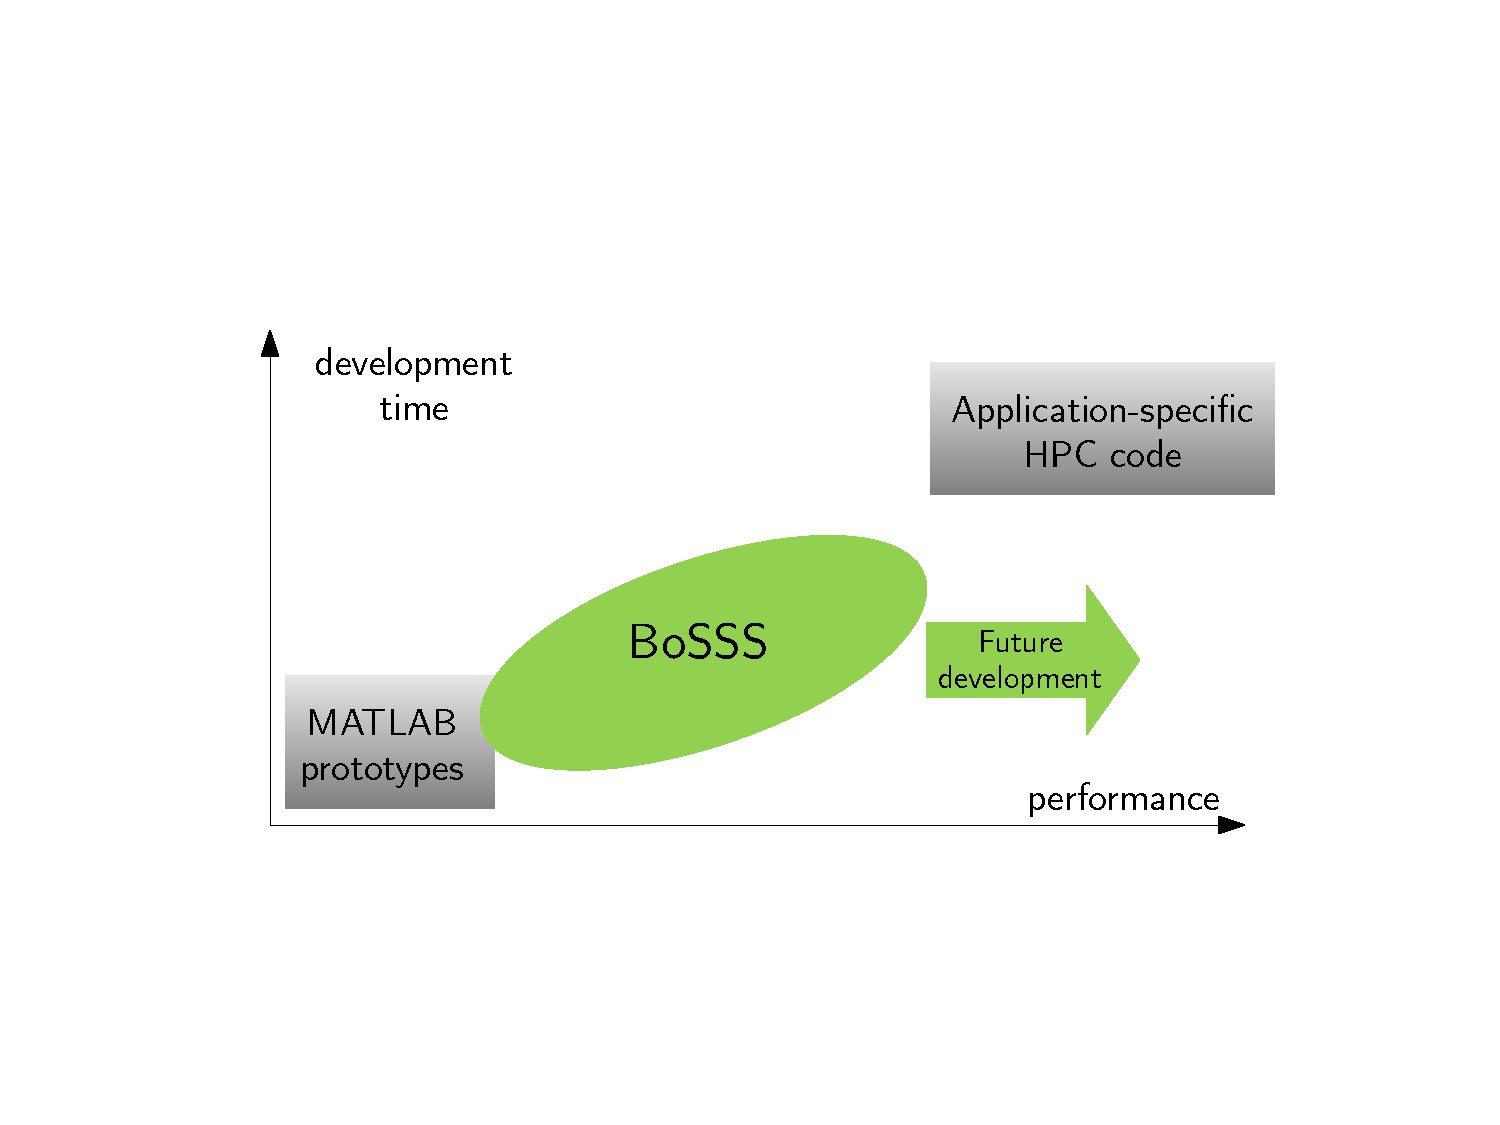
\includegraphics[width=0.8\textwidth]{figures/BoSSS-philosophy-2}
\end{center}
\caption{
While MATLAB prototypes are usually implemented quickly (at least for simple numerical methods)
they usually offer limited performance.
On the other side of the spectrum, there are application-specific high-performance codes,
tuned towards a specific physical problem.
The intention of \BoSSS{} is to bridge this gap: although it is slightly more difficult
than MATLAB,
%(general orientation of a new user in a new framework, C\# language is more complex than MATLAB scripts)
it offers higher performance and complete MPI parallelism.
}
\label{fig:BoSSS-Philosophy-2}
\end{figure}

\begin{figure}[!h]
\begin{center}
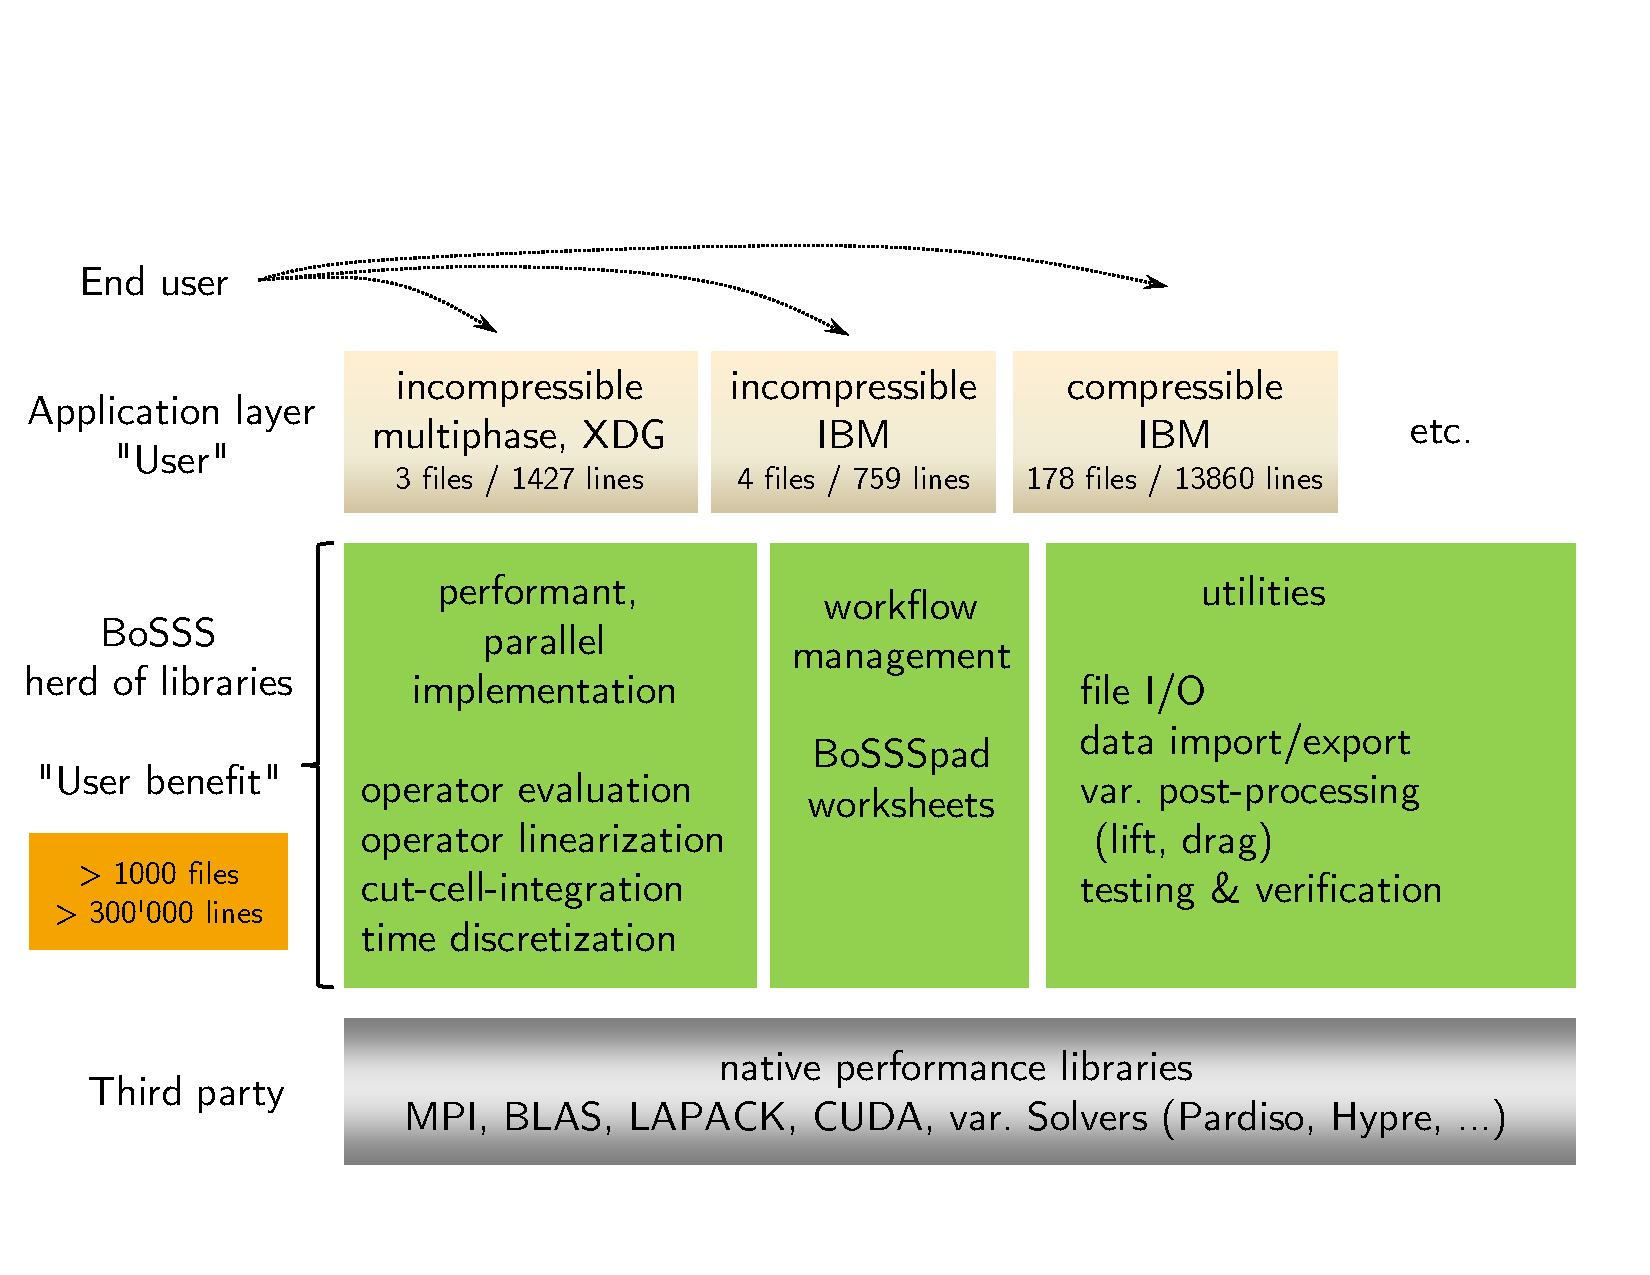
\includegraphics[width=0.85\textwidth]{figures/BoSSS-philosophy-1}
\end{center}
\caption{
BoSSS allows users to develop sophisticated solvers,
using e.g. eXtended discontinuous Galerkin (XDG)
or immersed boundary methods (IBM),
at a very low coding effort;
their benefit is three-fold: firstly, users can take advantage of the MPI-parallel,
performance-optimized operations for the evaluation of the DG operator, etc.;
secondly, users get access to highly customizable, yet proven workflow-management tools,
i.e. to \BoSSSpad{}; thirdly, users also profit from the existing utility codebase
for file I/O, data import and export (meshing and visualization) and a huge collection
of post-processing routines.
In addition to that, the user can rely that the operations he employs work correctly, due to the
sophisticated testing and verification environment.
}
\label{fig:BoSSS-Philosophy-1}
\end{figure}


\paragraph{Why C\#?}
While comparable software packages usually employ languages like
FORTRAN, C or C++, which are either very limited in terms of programming paradigms
or very hard to master for PhD students outside of computer science
(e.g. mechanical engineering),
BoSSS uses the C\#-language, which combines the
ease-of-use of Python with the execution speed of C or C++.
For a University-based research code, this is a quite unique feature.
The reason for the usage of 
FORTRAN, C or C++, sometimes in combination with Python scripts
in comparable software packages are, 
in our humble option, most of the time purely traditional.

The choice of C\#, on the other hand, is a key enabler for a series of interesting features:
For instance, a C\# program can be compiled once and executed everywhere. this means that a user can
develop and compile a code on her or his Mac or Windows laptop, and then execute
the code on a Linux-based supercomputer. This is obviously a great improvement
in comparison to a traditional HPC workflow, where the code has to be compiled and configured
for every computer separately. In addition, the compilation of C\# is also much faster than
C++ compilation - on a recent machine, the whole \BoSSS{} code
(more than 1000 files, 300'000 lines of code and 100'000 lines of comment)
can be compiled in less than half a minute.




\paragraph{Dynamic Interfaces:} 
A special feature of the \BoSSS{} code is its ability to treat dynamic (fluid) interfaces.
This is mainly used for two kinds of applications:
\begin{itemize}
\item
Immersed boundary methods: instead of creating a specialized mesh for a particular geometry,
the geometry is embedded in a simple background mesh.
An advantage of \ac{ibm} is that it is easy to implement moving geometries
(e.g. particle flows, fluid-structure interaction) since no mesh has to be moved.
See Figure \ref{fig:FlowOverBump} for a simple example.

\item
Multiphase flows: these are mixtures of at least two immiscible fluids, 
e.g. oil in water or water in air.
An example is the rising bubble simulation, shown in Figure \ref{fig:Bubbles}.

\end{itemize}


\begin{figure}[!h]
\begin{center}
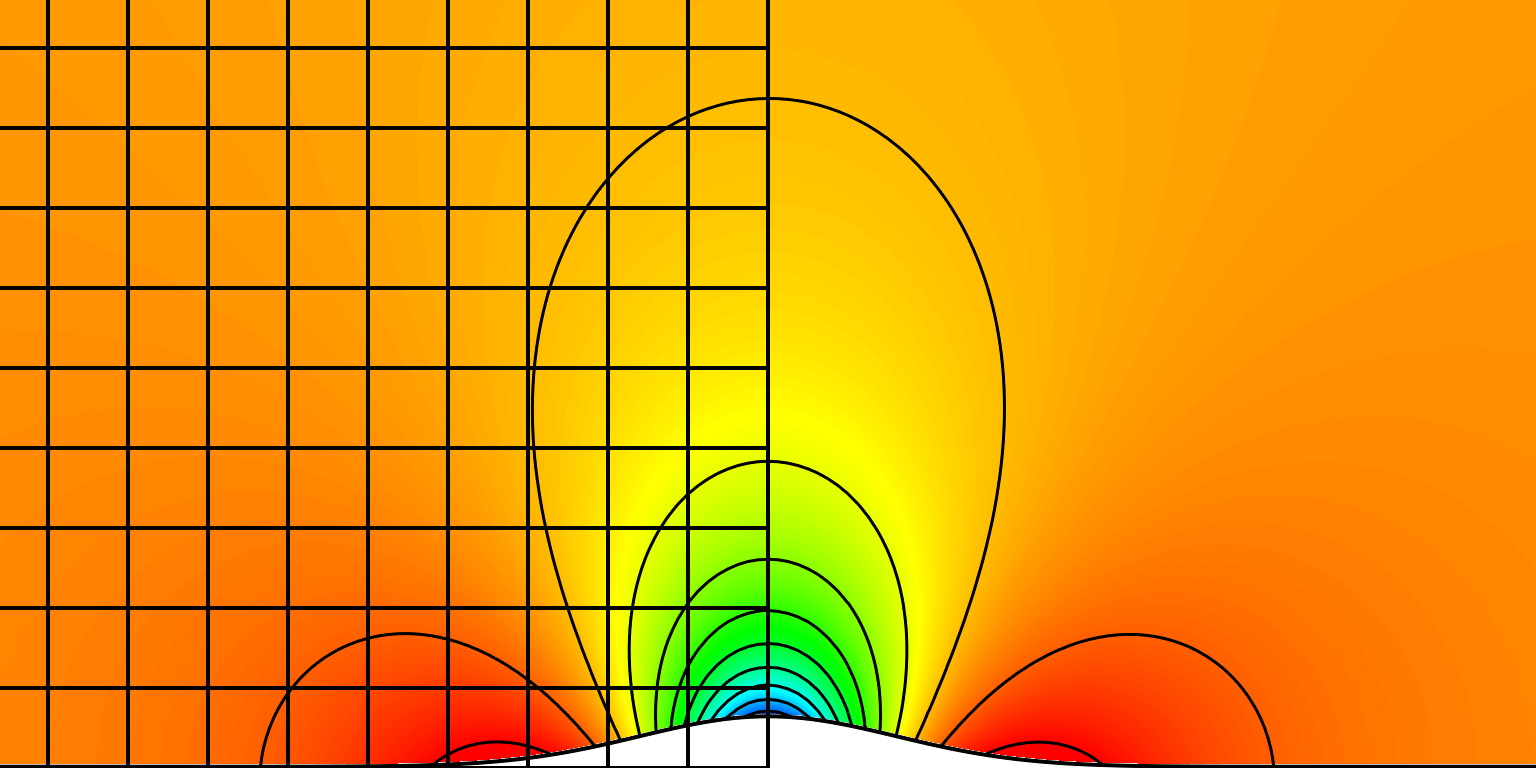
\includegraphics[width=0.65\textwidth]{figures/FlowOverBump2}
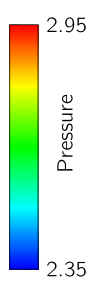
\includegraphics[width=0.09\textwidth]{figures/FlowOverBump2-legend}
\end{center}
\caption{
Compressible flow simulation over a Gaussian bump,
computed with \ac{ibm}. A Cartesian background mesh is used, 
and for the bum a so-called level-set representation is used.
}
\label{fig:FlowOverBump}
\end{figure}


\begin{figure}[!h]
\begin{center}
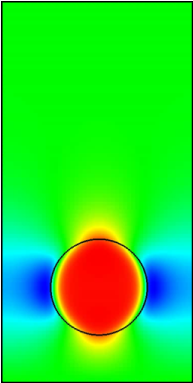
\includegraphics[width=0.2\textwidth]{figures/Bubble_t0}
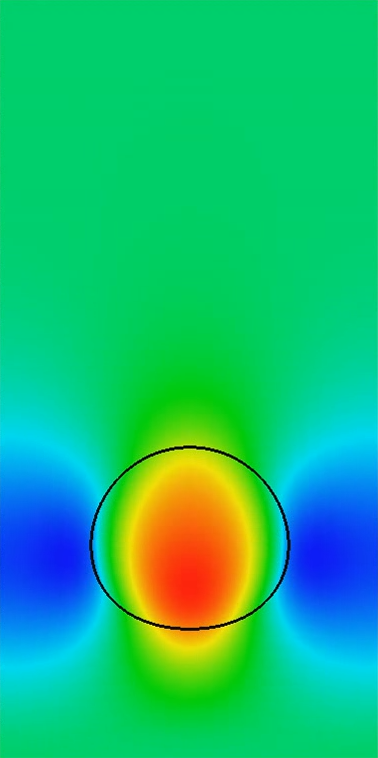
\includegraphics[width=0.2\textwidth]{figures/Bubble_t1}
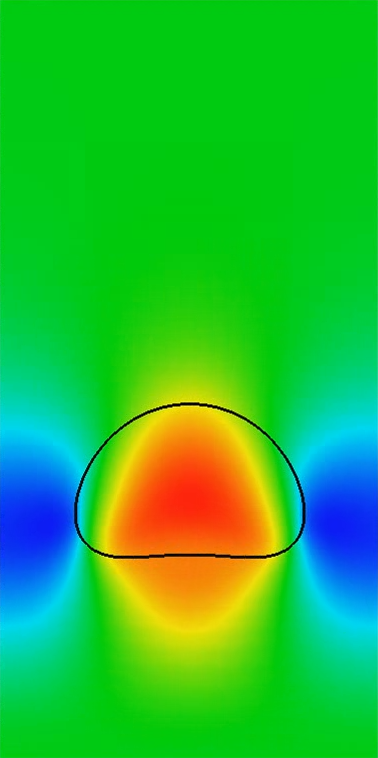
\includegraphics[width=0.2\textwidth]{figures/Bubble_t2}
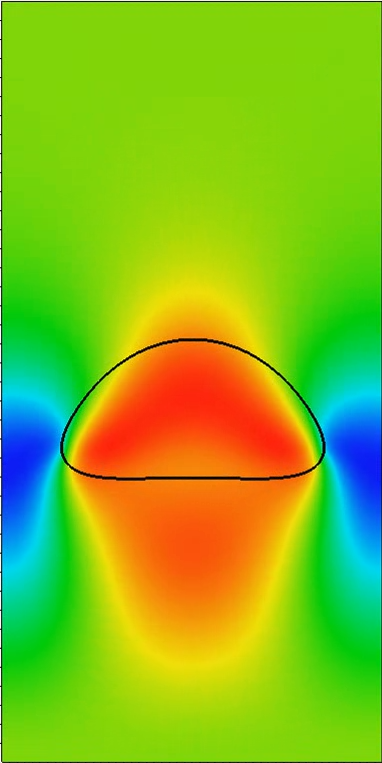
\includegraphics[width=0.2\textwidth]{figures/Bubble_t3}
\end{center}
\caption{
The second important application in \BoSSS{} using dynamic interfaces:
Incompressible multiphase simulation of a rising bubble.
}
\label{fig:Bubbles}
\end{figure}



% ################################################################################
\chapter{Core concepts}
\label{sec:coreConcepts}
% ################################################################################

This chapter covers certain issues in the design philosophy of the code, that are essential for its use. 
These are important to understand for both users as well as developers.

% --------------------------------------------------------------------------------
\section{Discontinuous Galerkin methods}
\label{sec:coreConcepts_dgMethods}
% --------------------------------------------------------------------------------
Obviously, in order to work with \BoSSS{} -- especially for the tutorial in part \ref{sec:Tutorial}
of this book -- one should have a basic understanding of \ac{dg} methods.
The purpose of this document is not to be (yet another) textbook on the \ac{dg} method.
As a reference, we recommend the textbook of \textcite{DiPietroErn2011},
as well as the lecture notes of Cockburn\footnote{
\url{http://www-users.math.umn.edu/~bcockbur//LectureNotes.html}}
and Hartmann\footnote{
\url{http://numerik.iwr.uni-heidelberg.de/~hartmann/publications/publications.html\#lectures}}.

(Remark: at some point, this document might be extended with a mathematical
reference on the specific version of the \ac{dg} method in \BoSSS; this may cover e.g.
details on the specific, modal \ac{dg} basis, indexing conventions, etc.)


% --------------------------------------------------------------------------------
\section{C\#, .NET and Mono}
\label{sec:coreConcepts_CsharpAndDotnet}
% --------------------------------------------------------------------------------
\BoSSS{} is written in the \emph{programming language} C\#, which is compiled into the so-called 
\emph{Common Intermediate Language} (CIL). CIL-code is platform independent and can be executed (without recompilation) 
on any platform where an implementation of the standardized \emph{Common Language Infrastructure} (CLI) is available. 
Examples include Windows (using the .NET framework), Linux and Mac OS X (both using the mono framework). 
Almost all parts of \BoSSS{} are thus platform-independent and directly be used after obtaining the \BoSSS{} binaries 
and a platform-specific CLI implementation (cf. Section \ref{sec:gettingStarted_installation}).

Like for any other language, a C\# program needs to be compiled. Any C\# compiler produces executable 
files (ending with \texttt{.exe}) that typically rely on library files (ending with \texttt{.dll}). 
In contrast to languages like C, the executables cannot be executed directly -- they need to be executed
 through the CLI which compiles the CIL to machine code \emph{at runtime}. Due to this \emph{just in time} (JIT) 
compilation, C\# is able to compete with compiled languages in terms of performance.

This two-step compile approach makes C\# a fast language -- cooperatively fast to 
languages like C or FORTRAN. C\# is significantly faster than an interpreted language like 
Matlab or Phython. 

The .NET framework is very tightly integrated with Windows, so that it is almost transparent to the user. 
While a .NET-executable is internally fundamentally different from a standard executable, it behaves very similar 
and can be executed by the user via a simple double-click. Windows detects which kind of \texttt{.exe} file is 
at hand and uses .NET if necessary. .NET is also omnipresent on Windows -- it is almost impossible to find a 
Windows computer without,
since it is used for many applications.

On Linux or MacOS, however, there is no such shortcut, which is why the user has to execute \texttt{.exe} 
files via mono by hand. For example, the \BoSSSpad{} application \texttt{BoSSSpad.exe} 
(see Section \ref{sec:coreConcepts_BoSSSpad}) is started

\code{mono BoSSSpad.exe \$commandLineArgumentsForBoSSSpad}

This command makes Mono load the \texttt{.exe} file, translate it into machine code for the respective 
operating system, and finally execute this machine code.
Note also C\# programs are always compiled into {\tt .exe} files, even on Linux or MacOS,
which seems unusual for these operating systems. 

Finally, we note that traditional languages like C differentiate between compiling and linking, whereas 
C\# always performs both steps are done at once.
(Although one could philosophize on this, since 
modern compilers like {\tt gcc} can do both, compiling and linking
in one step or separately.)


% --------------------------------------------------------------------------------
\section{Compile once -- Run everywhere: using High Performance Computing systems}
\label{sec:HPCuse}
% --------------------------------------------------------------------------------
The use of \BoSSS{} on \ac{hpc} systems is a bit \emph{more convenient} than other 
research codes.
Unusually, such codes have to be compiled for each system individually. 
The advantage of C\#, resp. .NET is that \emph{the executable is platform-independent}.

That means e.g. that an executable which was compiled on a Windows or Mac laptop can be copied 
to a \ac{hpc} system, which usually runs some breed of Linux, and be executed there without re-compilation.
This, of course requires some middleware (the Mono framework, see section \ref{sec:coreConcepts_CsharpAndDotnet})
and libraries to be present on the target computer.

In addition to C\# code,  \BoSSS{} relies on platform-specific ('\emph{native}') third party libraries for specific tasks, 
such as MPI for parallelization and BLAS/LAPACK for high-performance linear algebra. In 
section \ref{sec:gettingStarted_installation}, we will thus 
=========
such MPI for parallelization and BLAS/LAPACK for high-performance linear algebra. In 
section \ref{sec:gettingStarted_installation}, we will thus 
summarize some best practices for the installation of \BoSSS{} on different operating systems.

Once the required libraries and middleware for \BoSSS{} have been installed on an 
\ac{hpc} system, all simulation set-up and development can be done 
on a user's local machine.
This is advantageous, since the development tools on \ac{hpc} systems are usually limited
(users have to live with what administrators provide)
and have to be used through an ssh-connection.
(This can be especially annoying when working with laptops in unreliable WiFi-environments,
where ssh-sessions crash on a regular basis, or have a noticeable lag.)

% --------------------------------------------------------------------------------
\section{Workflow management: database and the \BoSSSpad}
\label{sec:coreConcepts_BoSSSpad}
% --------------------------------------------------------------------------------
Since the \BoSSS{} code is essentially a research-project, therefore 
tools with a \ac{gui}  are limited.

However, also for research codes  one faces the challenge of performing 
e.g. parameter studies with which involve thousands of individual 
solver runs.
Therefore, some management tools are inevitable, since manual or semi-automated
organization of simulation result using usual operating system tools (e.g. 
directory structures, shell scripts, etc.) have proven to be error-prone.

In \BoSSS{}, these issues are managed using two components:
\begin{itemize}
\item
A database for \emph{data management}:
all simulation data, together with configuration files, etc., are stored automatically.
Technically, the database is set of files and directories, following 
certain internal conventions.

\item
A sophisticated scripting solution for \emph{workflow management}, the \BoSSSpad{} application:
C\# is not only used as a programming language, but also as a scripting language
for setting up simulations and examining results.

In \BoSSSpad{}, users can enter C\# statements and execute them on the fly.
Since C\# is used for both, the code development as well as scripting,
the user can seamlessly access every subroutine of the code.

\begin{itemize}
\item
Access and manage the database

\item
Workflow management: launch solvers, submit jobs to hpc systems, ...

\item
Data import and export: load data from third-party pre-processing tools (mesh generators),
export to post-processing tools (visualization software).

\item
Rapid prototyping of (new) \ac{dg} solvers: the tutorials in part \ref{sec:Tutorial} demonstrate this.

\item
Analysis and post-processing: some analysis tasks, e.g. lift and drag computation,
can be done directly in \BoSSSpad{}.

\item
Documentation and tutorials: 
since \BoSSSpad{} can also produce \LaTeX output, it can also be used to 
build nicely formatted tutorials, as e.g. found in  part \ref{sec:Tutorial} of this book.

\end{itemize}
\end{itemize}
A typical workflow using these two components is shown in Figure \ref{fig:BoSSS-workflow}.

\begin{figure}
  \begin{center}
  \begin{overpic}[width=0.9\textwidth%,grid,tics=10
  ]{figures/BoSSS-workflow}
  \put(-2.5,23) {\parbox{2.8cm}{\centering Mesh file \\ e.g. {\tt gmsh }}}
  \put(84.2,21.5) {\parbox{2.8cm}{\centering Output files \\ e.g. Tecplot}}
  \put(38,9.0) {\parbox{3.3cm}{\centering\Large \BoSSS{} database}}
  \put(43,60) {\Large \BoSSSpad}
  \put(38,40) {\parbox{3.2cm}{\centering some solver, e.g. {\tt CNS.exe} (compressible, see chapter \ref{CNS})}}
  \put(76.5,40) {\parbox{3.2cm}{\centering plot generator tool (or other post-processing)}}
  \put(78,10.5) {data reading}
  \put(78,5.5)  {data writing}
  \put(78,0)    {program launch}
  \put(36,1.5)  {HPC system (optional)}
  \put(0,55)    {\parbox{3cm}{\centering (1) import mesh file      }}
  \put(7.7,40)   {\parbox{2.8cm}{\centering (2) save mesh \\ in database }}
  \put(48,53)   {(3) launch solver}
  \put(37,27)   {\parbox{3.3cm}{\centering (4) solver reads mesh, writes results}}
  \put(73,56.2) {(5) launch post-processing}
  \put(66.5,20)   {\parbox{3cm}{\centering (6) plot generator reads results \& exports files for visualization}}
  \end{overpic}
 \end{center}
\caption{
An exemplary workflow in \BoSSS{} where everything is controlled by \BoSSSpad{}.
All relevant data is stored in the database.
From \BoSSSpad{}, one could import a computational mesh, which has been created 
using a third-party tool, e.g. {\tt gmsh};
This data is imported into \BoSSS{} 
(via the function \code{GridImporter.Import})
and saved in the \BoSSS{} database (using \code{IDatabaseDriver.SaveGridIfUnique}).
The workflow management tools (see chapter \ref{sec:WorkflowMgm}) of \BoSSSpad
can then be used to launch one of the provided solvers, which also save their results to the database.
Finally, \BoSSSpad{} ~can also be used to launch post-processing or data export tools.
The solver as well as the database can optionally be located/run on some other 
computer, e.g. some sort of High Performance Compute (HPC) system.
}
\label{fig:BoSSS-workflow}
\end{figure}


\emph{Warning: do not try to manipulate the files in the database manually!} 
One should always use \BoSSSpad{} to work with the database -- the essential commands can be found
e.g. in part \ref{sec:BoSSSpadReference}.



% --------------------------------------------------------------------------------
\section{Pre-compiled or source: end-user vs. developer}
% --------------------------------------------------------------------------------
\label{sec:coreConcepts_using}
The \BoSSS{} can be used in two ways: As a binary distribution and in the form of source code.
One can start in one of the following ways:
\begin{itemize}
\item
\emph{Pre-compiled version:}
One may start using existing solvers
(e.g. \code{CNS} for compressible or \code{INS} for incompressible Navier-Stokes).
This is the classical \emph{end-user scenario} and requires only the binary distribution.
As a workflow management tool, the \BoSSSpad{} application 
(see section \ref{sec:coreConcepts_BoSSSpad})
is recommended; 
alternatively, one may launch a solver from command line.

\item
\emph{Scripting:}
Also if one wants to obtain deeper insights into the methodology of \ac{dg},
the \code{BoSSSpad} may be a good starting point.
Since it can be utilized to access almost every subroutine of the \BoSSS{} software libraries,
it is not only usable as a workflow management tool, 
but can also be used to develop new solvers.
This requires basic knowlege of C\#-programming.
The tutorials in this handbook, for instance, were exclusively
created using the \BoSSSpad{}.

\item
\emph{Working with source code:}
The most advanced way of working with the \BoSSS{} code is obviously
working with source code itself.
For instance, if one wants to implement a turbulence model or a completely new solver 
for an equation that is not covered by the existing solvers.
This is a \emph{developer scenario}. 
This requires profound knowledge of C\#-programming and the 
associated development environments (e.g. Visual Studio or equivalents).

\end{itemize}


% ********************************************************************************
% ********************************************************************************
\chapter{Getting started}
\label{sec:gettingStarted}
% ********************************************************************************
% ********************************************************************************

Within this chapter, we will briefly outline the steps required to get started with using and/or developing \BoSSS{} applications. In any case, the installation of the pre-compiled version of \BoSSS{} (cf. section \ref{sec:gettingStarted_installation}) should be the first step. Upon finishing this step, you will be able to use the pre-compiled \BoSSS{} applications (cf. section \ref{sec:gettingStarted_using}), but also to start  exploring the code using the scripting API. Finally, working with the source code will be discussed in section \ref{sec:gettingStarted_developing}.

% --------------------------------------------------------------------------------
\section{Installation}
\label{sec:gettingStarted_installation}
% --------------------------------------------------------------------------------
The advantage of C\#, resp. .NET is that \emph{the executable is platform-independent}. This implies that an executable compiled on a Windows/Mac laptop can be copied to a Linux/Unix \ac{hpc} system and executed there without re-compilation. As discussed in section \ref{sec:coreConcepts_CsharpAndDotnet}, this obviously requires some \emph{middleware} and some libraries to be present on the target computer. In the following, we will thus summarize some best practices for the installation of the pre-compiled \BoSSS{} binaries\footnote{\label{note:relases} \url{https://github.com/FDYdarmstadt/BoSSS/releases}} on different operating systems.

\subsection{Windows}
Installation on Windows is quite straightforward because the \BoSSS{} installer already includes all required native libraries:
\begin{enumerate}
	\item Ensure that the .NET framework\footnote{\url{https://www.microsoft.com/net/download/framework}} (version .NET 4.5.2 or higher) is installed 
	\item Download and install Microsoft MPI\footnote{\url{https://msdn.microsoft.com/en-us/library/bb524831(v=vs.85).aspx})}. Check the MPI installation by executing the command \texttt{mpiexec} in a console window
	\item Obtain and execute the \BoSSS{} Windows installer
	\item Test your installation (cf. section \ref{sec:installation_testing})
\end{enumerate}

\paragraph{Known issues:}
The .NET framework is shipped with two JIT compilers that compile the CIL to machine code at runtime (cf. section \ref{sec:coreConcepts_CsharpAndDotnet}). One of these, \emph{RyuJIT}, contains a bug that causes \BoSSS{} applications to crash with misleading error messages, typically related to grid handling. RyuJIT should thus be deactivated\footnote{\url{https://github.com/Microsoft/dotnet/blob/master/Documentation/testing-with-ryujit.md}} when using \BoSSS{} on Windows.


\subsection{Linux}
In the following, we thus focus on the installation of \BoSSS{} itself. 
The \BoSSS{} group does not maintain packages of the native libraries listed in section \ref{sec:installation_libraries} for Linux because high-performance computers typically provide specifically optimized versions of these libraries that should be used in order to obtain optimal performance. 

\begin{itemize}
	\item Obtain Mono\footnote{\url{www.mono-project.com}} (version 3.0 or higher), either by installing a pre-built package\footnote{\url{www.mono-project.com/download/}} or by compiling\footnote{\url{www.mono-project.com/docs/compiling-mono/linux/}} it from a tarball\footnote{\url{https://download.mono-project.com/sources/mono/}}
	\item Obtain/install/load OpenMPI (tested with version 1.6.5 and higher)
	\item Obtain/install/load BLAS and LAPACK (tested with AMD Core Math Library 5.3.1)
	\item Test your basic installation (cf. section \ref{sec:installation_testing})
	\item Obtain/install/load additional libraries if required by the particular \BoSSS{} application
\end{itemize}


\paragraph{Known issues:}
One some system (tested with CentOS 7), current versions of Mono (versions 5 and higher), the error message
\begin{verbatim}
Got a bad hardware address length for an AF_PACKET 20 8
\end{verbatim}
may appear. This seems to be an inconsequential bug in Mono that can safely be ignored.


\subsection{Mac OS X}
Support for Mac OS X will follow soon.


\section{Testing the installation}
\label{sec:installation_testing}

\code{BoSSSpad.exe --check}


\subsection{Third-party libraries}
\label{sec:installation_libraries}

\BoSSS{} tries to load these libraries dynamically
\begin{itemize}
	\item MPI: Parallelization
	\item BLAS
	\item LAPACK
	\item Optional: ParMETIS
	\item Optional: Tecplot
	\item Optional: CGNS
	\item Optional: MUMPS
\end{itemize}


% --------------------------------------------------------------------------------
\section{Using \BoSSS{}}
\label{sec:gettingStarted_using}
% --------------------------------------------------------------------------------

Having familiarized with the core concepts of \BoSSS{} (cf. chapter \ref{sec:coreConcepts}) and verified that the installation was succesfull (cf. section \ref{sec:installation_testing}), the pre-compiled solvers shipped with \BoSSS{} can be used to solve compressible as well as incompressible flow problems. The most simple way to get a feeling for the usage of the different solvers is to follow the corresponding quick start guides given in section \ref{sec:quickStartGuides}. These guides have been structured such that they allow new users to get first results immediately, which is why details about certain concepts are left out. These will then be discussed in depth in the tutorials given in part \ref{sec:Tutorial}.


\subsection{\BoSSSpad{}}

\code{}

\subsection{\BoSSS{} applications}




% --------------------------------------------------------------------------------
\section{As a developer}
\label{sec:gettingStarted_developing}
% --------------------------------------------------------------------------------

Even if you want to compile \BoSSS{} yourself, we \emph{strictly recommend} that
you \emph{install the binary distribution first}.


\subsection{Development Tools}
As every software developer knows, programming is either done by using a 
command line tool-chain or with an \ac{ide}. We strongly recommend the latter 
approach.

\paragraph{Development Environments}
The major \ac{ide}s available for C\# are 
Microsoft Visual Studio\footnote{
\url{https://www.visualstudio.com/downloads/}},
Xamarin Studio (also known under its former name `Monodevelop' or as `Visual Studio for Mac')\footnote{
\url{http://www.monodevelop.com}}
and SharpDevelop\footnote{
\url{http://www.icsharpcode.net/OpenSource/SD/Default.aspx}}.
Note: `Visual Studio' should not be confused with `Visual Studio Code'. The latter is more an editor
than an \ac{ide}.

On Windows, we strongly recommend to use the latest version of Visual Studio.
The Community Edition can be downloaded for free.
Alternatively, one could also use either Xamarin Studio or SharpDevelop.
In those environments, the integrated debugger cannot be used for \BoSSS{}:
The native libraries for BoSSS on Windows are only provided for  
64 bit (AMD64 resp. X86\_64 architecture), therefore \BoSSS{} has to be debugged in 64 bit mode.
Xamarin Studio and SharpDevelop do not support 64 bit debugging, so they cannot be used to
debug \BoSSS{}.
This issue renders them significantly inferior to Visual Studio.

On Linux, however, Xamarin Studio supports 64 bit and can therefore be used without any restriction.
If possible, we recommend to use the latest version of Xamarin Studio from
the official and not the version from the Linux distributions package management system,
since these are very often out-dated (still called Monodevelop).

On Mac OS, one certainly should use Xamarin Studio, resp. Visual Studio for Mac.

\paragraph{Command line toolchain}
Of course, \BoSSS{} can also be developed in the traditional way, 
by using a text editor of choice and a command-line build tool.

If .NET is used, the build tool is {\tt msbuild}.
The main solution file of \BoSSS{} could be compiled e.g. by
\[
 \mathtt{msbuild} \ \text{\tt Public.sln} \ \text{\tt /p:Configuration=Debug /p:Platform="Any CPU"}
\]
in Debug mode (runs slower, more tests, for development and debugging) and by
\[
 \mathtt{msbuild} \ \text{\tt Public.sln} \  \text{\tt /p:Configuration=Release /p:Platform="Any CPU"}
\]
in Release mode (runs faster, less tests, designated for production runs).

When Mono is used, the equivalent to {\tt msbuild} is {\tt xbuild}. Both tools have the same syntax.



% ################################################################################
% ################################################################################
% ################################################################################
\part{End-user tutorials}
\label{sec:quickStartGuides}
% ################################################################################
% ################################################################################
% ################################################################################

% ################################################################################
\chapter{Compressible Navier-Stokes (CNS) Solver }
\label{CNS}
% ################################################################################
\import{./quickStartCNS/}{IsentropicVortex.tex}

% ################################################################################
\chapter{Workflow management and meta job scheduler}
\label{sec:WorkflowMgm}
% ################################################################################
\import{./MetaJobManager/}{MetaJobManager.tex}

% ################################################################################
\chapter{Incompressible Navier-Stokes Solver}
\label{IBM}
% ################################################################################
\import{./quickStartIBM/}{channel.tex}

% ################################################################################
% ################################################################################
% ################################################################################
\part{Developer tutorials}
\label{sec:Tutorial}
% ################################################################################
% ################################################################################
% ################################################################################

% ################################################################################
\chapter{Interface for Matlab using the BatchmodeConnector}
\label{Matlab}
% ################################################################################
\import{./shortTutorialMatlab/}{tutorialMatlab.tex}

% ################################################################################
\chapter{Grid instantiation, $L^2$-projection and convergence}
\label{GridInstantiation}
% ################################################################################
\import{./tutorial2/}{uebung2tutorial.tex}


% ################################################################################
\chapter{Defining a Spatial Operator and using explicit time integration}
\label{SpatialOperator}
% ################################################################################
\import{./tutorial4/}{tutorial4.tex}


% ################################################################################
\chapter{Numerical flux and convergence study}
\label{NumFlux}
% ################################################################################
\import{./tutorial5/}{uebung5tutorial.tex}


% ################################################################################
\chapter{Scalar convection and stability of explicit timesteppers}
\label{ScalarAdvection}
% ################################################################################
\import{./tutorial6/}{tutorial6.tex}

%\chapter{Exporting data}
%\chapter{Working with masks and subgrids}
%\chapter{Hyperbolic systems}
%\chapter{Second order operators, implicit}




% ################################################################################
\chapter{Poisson equation using the Symmetric Interior Penalty method}
% ################################################################################
\label{sec:SIP}
\import{./tutorial9-SIP/}{sip.tex}

% ################################################################################
\chapter{Poisson equation as a System}
\label{sec:PoissonAsASystem}
% ################################################################################
\import{./tutorial10-PoissonSystem/}{Poisson.tex}

% ################################################################################
\chapter{Stokes equation}
\label{sec:Stokes}
% ################################################################################
\import{./tutorial11-Stokes/}{StokesEq.tex}



% ################################################################################
% ################################################################################
% ################################################################################
\part{Appendix}
\appendix
% ################################################################################
% ################################################################################
% ################################################################################

% ################################################################################
\chapter{Single Node Performance}
\label{sec:SingleNodePerformance}
% ################################################################################
This section covers basic performance tests, i.e. how specific algorithms scale 
with grid resolution or with polynomial degree, on a \emph{single compute node}.

% --------------------------------------------------------------------------------
\section{Solver Performance - Poisson problems}
\label{sec:SolverPerformancePoisson}
% --------------------------------------------------------------------------------
Three different groups of solvers are compared:
\begin{itemize}
\item
Direct Solvers: directs sparse methods, such as PARDISO\footnote{
\url{http://www.pardiso-project.org/}}
and MUMPS\footnote{
\url{http://mumps.enseeiht.fr/}}
are compared.
Their performance also serves as a comparative baseline.

\item
Iterative Algorithms without preconditioning, resp. low-impact, generic preconditioning:
This includes solver libraries such as \code{monkey} (BoSSS-specific, supports GPU)
as well as 
HYPRE\footnote{
\url{https://computation.llnl.gov/projects/hypre-scalable-linear-solvers-multigrid-methods}}
(native library, used via wrappers).

\item
Iterative Algorithms with \ac{dg}-specific preconditioners, such as aggregation multigrid
and multi-level additive Schwarz
\end{itemize}

\subsection{Problems with Constant Diffusion Coefficient}
\label{sec:ConstantDiffusionCoefficient}
The problem
\begin{equation}
\left\{ \begin{array} {rclll}
- \Delta T   & = & g_{\domain}                      
             & \text{in}\ \Omega = (0,10) \times (-1,1) \times (-1,1)  &  \\
% ----
         T   & = & g_D = 0                             
             & \text{on}\ \Gamma_D = \{ (x,y,z) \in \real^3; \ x = 0 \}
             & \text{Dirichlet-boundary} \\
% ----
\nabla T \cdot \vec{n}_{\partial \domain} & = & g_N 
             & \text{on}\ \Gamma_N = \partial \Omega \setminus \Gamma_D
             & \text{Neumann-boundary}
\end{array} \right.
\label{eq:ContantCoeffPoissonBenchmark}
\end{equation}
is investigated on a non-uniform, Cartesian grid
(equidistant in $z$, sinus-spacing in $x$ and $y$ direction).
The large $\Gamma_N$ makes the problem harder for non-preconditioned
iterative methods. See Figure \ref{fig:ConstantCoeffRuntimes} for results.

\graphicspath{{./apdx-NodeSolverPerformance/PoissonConstCoeff/plots/}}

\begin{figure}[!h]
\begin{center}
% GNUPLOT: LaTeX picture with Postscript
\begingroup
  \makeatletter
  \providecommand\color[2][]{%
    \GenericError{(gnuplot) \space\space\space\@spaces}{%
      Package color not loaded in conjunction with
      terminal option `colourtext'%
    }{See the gnuplot documentation for explanation.%
    }{Either use 'blacktext' in gnuplot or load the package
      color.sty in LaTeX.}%
    \renewcommand\color[2][]{}%
  }%
  \providecommand\includegraphics[2][]{%
    \GenericError{(gnuplot) \space\space\space\@spaces}{%
      Package graphicx or graphics not loaded%
    }{See the gnuplot documentation for explanation.%
    }{The gnuplot epslatex terminal needs graphicx.sty or graphics.sty.}%
    \renewcommand\includegraphics[2][]{}%
  }%
  \providecommand\rotatebox[2]{#2}%
  \@ifundefined{ifGPcolor}{%
    \newif\ifGPcolor
    \GPcolortrue
  }{}%
  \@ifundefined{ifGPblacktext}{%
    \newif\ifGPblacktext
    \GPblacktexttrue
  }{}%
  % define a \g@addto@macro without @ in the name:
  \let\gplgaddtomacro\g@addto@macro
  % define empty templates for all commands taking text:
  \gdef\gplbacktext{}%
  \gdef\gplfronttext{}%
  \makeatother
  \ifGPblacktext
    % no textcolor at all
    \def\colorrgb#1{}%
    \def\colorgray#1{}%
  \else
    % gray or color?
    \ifGPcolor
      \def\colorrgb#1{\color[rgb]{#1}}%
      \def\colorgray#1{\color[gray]{#1}}%
      \expandafter\def\csname LTw\endcsname{\color{white}}%
      \expandafter\def\csname LTb\endcsname{\color{black}}%
      \expandafter\def\csname LTa\endcsname{\color{black}}%
      \expandafter\def\csname LT0\endcsname{\color[rgb]{1,0,0}}%
      \expandafter\def\csname LT1\endcsname{\color[rgb]{0,1,0}}%
      \expandafter\def\csname LT2\endcsname{\color[rgb]{0,0,1}}%
      \expandafter\def\csname LT3\endcsname{\color[rgb]{1,0,1}}%
      \expandafter\def\csname LT4\endcsname{\color[rgb]{0,1,1}}%
      \expandafter\def\csname LT5\endcsname{\color[rgb]{1,1,0}}%
      \expandafter\def\csname LT6\endcsname{\color[rgb]{0,0,0}}%
      \expandafter\def\csname LT7\endcsname{\color[rgb]{1,0.3,0}}%
      \expandafter\def\csname LT8\endcsname{\color[rgb]{0.5,0.5,0.5}}%
    \else
      % gray
      \def\colorrgb#1{\color{black}}%
      \def\colorgray#1{\color[gray]{#1}}%
      \expandafter\def\csname LTw\endcsname{\color{white}}%
      \expandafter\def\csname LTb\endcsname{\color{black}}%
      \expandafter\def\csname LTa\endcsname{\color{black}}%
      \expandafter\def\csname LT0\endcsname{\color{black}}%
      \expandafter\def\csname LT1\endcsname{\color{black}}%
      \expandafter\def\csname LT2\endcsname{\color{black}}%
      \expandafter\def\csname LT3\endcsname{\color{black}}%
      \expandafter\def\csname LT4\endcsname{\color{black}}%
      \expandafter\def\csname LT5\endcsname{\color{black}}%
      \expandafter\def\csname LT6\endcsname{\color{black}}%
      \expandafter\def\csname LT7\endcsname{\color{black}}%
      \expandafter\def\csname LT8\endcsname{\color{black}}%
    \fi
  \fi
    \setlength{\unitlength}{0.0500bp}%
    \ifx\gptboxheight\undefined%
      \newlength{\gptboxheight}%
      \newlength{\gptboxwidth}%
      \newsavebox{\gptboxtext}%
    \fi%
    \setlength{\fboxrule}{0.5pt}%
    \setlength{\fboxsep}{1pt}%
\begin{picture}(7920.00,6800.00)%
    \gplgaddtomacro\gplbacktext{%
      \csname LTb\endcsname%
      \put(997,4825){\makebox(0,0)[r]{\strut{}$10^{-2}$}}%
      \csname LTb\endcsname%
      \put(997,5150){\makebox(0,0)[r]{\strut{}$10^{-1}$}}%
      \csname LTb\endcsname%
      \put(997,5475){\makebox(0,0)[r]{\strut{}$10^{0}$}}%
      \csname LTb\endcsname%
      \put(997,5800){\makebox(0,0)[r]{\strut{}$10^{1}$}}%
      \csname LTb\endcsname%
      \put(997,6126){\makebox(0,0)[r]{\strut{}$10^{2}$}}%
      \csname LTb\endcsname%
      \put(997,6451){\makebox(0,0)[r]{\strut{}$10^{3}$}}%
      \csname LTb\endcsname%
      \put(997,6776){\makebox(0,0)[r]{\strut{}$10^{4}$}}%
      \csname LTb\endcsname%
      \put(1099,4646){\makebox(0,0){\strut{} }}%
      \csname LTb\endcsname%
      \put(2137,4646){\makebox(0,0){\strut{} }}%
      \csname LTb\endcsname%
      \put(3176,4646){\makebox(0,0){\strut{} }}%
      \csname LTb\endcsname%
      \put(4214,4646){\makebox(0,0){\strut{} }}%
      \csname LTb\endcsname%
      \put(5252,4646){\makebox(0,0){\strut{} }}%
      \csname LTb\endcsname%
      \put(6291,4646){\makebox(0,0){\strut{} }}%
      \csname LTb\endcsname%
      \put(7329,4646){\makebox(0,0){\strut{} }}%
      \csname LTb\endcsname%
      \put(7431,4825){\makebox(0,0)[l]{\strut{} }}%
      \csname LTb\endcsname%
      \put(7431,5150){\makebox(0,0)[l]{\strut{} }}%
      \csname LTb\endcsname%
      \put(7431,5475){\makebox(0,0)[l]{\strut{} }}%
      \csname LTb\endcsname%
      \put(7431,5801){\makebox(0,0)[l]{\strut{} }}%
      \csname LTb\endcsname%
      \put(7431,6126){\makebox(0,0)[l]{\strut{} }}%
      \csname LTb\endcsname%
      \put(7431,6451){\makebox(0,0)[l]{\strut{} }}%
      \csname LTb\endcsname%
      \put(7431,6776){\makebox(0,0)[l]{\strut{} }}%
    }%
    \gplgaddtomacro\gplfronttext{%
      \csname LTb\endcsname%
      \put(397,5800){\rotatebox{-270}{\makebox(0,0){\strut{}$k = 2$}}}%
      \csname LTb\endcsname%
      \put(2190,6565){\makebox(0,0)[l]{\strut{}GMRES w. pTG}}%
      \csname LTb\endcsname%
      \put(2190,6286){\makebox(0,0)[l]{\strut{}Kcycle w. add.-Schwarz}}%
      \csname LTb\endcsname%
      \put(2190,6007){\makebox(0,0)[l]{\strut{}Pardiso}}%
      \csname LTb\endcsname%
      \put(2190,5728){\makebox(0,0)[l]{\strut{}linear}}%
    }%
    \gplgaddtomacro\gplbacktext{%
      \csname LTb\endcsname%
      \put(997,2558){\makebox(0,0)[r]{\strut{}$10^{-2}$}}%
      \csname LTb\endcsname%
      \put(997,2883){\makebox(0,0)[r]{\strut{}$10^{-1}$}}%
      \csname LTb\endcsname%
      \put(997,3209){\makebox(0,0)[r]{\strut{}$10^{0}$}}%
      \csname LTb\endcsname%
      \put(997,3534){\makebox(0,0)[r]{\strut{}$10^{1}$}}%
      \csname LTb\endcsname%
      \put(997,3859){\makebox(0,0)[r]{\strut{}$10^{2}$}}%
      \csname LTb\endcsname%
      \put(997,4185){\makebox(0,0)[r]{\strut{}$10^{3}$}}%
      \csname LTb\endcsname%
      \put(997,4510){\makebox(0,0)[r]{\strut{}$10^{4}$}}%
      \csname LTb\endcsname%
      \put(1099,2379){\makebox(0,0){\strut{} }}%
      \csname LTb\endcsname%
      \put(2137,2379){\makebox(0,0){\strut{} }}%
      \csname LTb\endcsname%
      \put(3176,2379){\makebox(0,0){\strut{} }}%
      \csname LTb\endcsname%
      \put(4214,2379){\makebox(0,0){\strut{} }}%
      \csname LTb\endcsname%
      \put(5252,2379){\makebox(0,0){\strut{} }}%
      \csname LTb\endcsname%
      \put(6291,2379){\makebox(0,0){\strut{} }}%
      \csname LTb\endcsname%
      \put(7329,2379){\makebox(0,0){\strut{} }}%
      \csname LTb\endcsname%
      \put(7431,2558){\makebox(0,0)[l]{\strut{} }}%
      \csname LTb\endcsname%
      \put(7431,2883){\makebox(0,0)[l]{\strut{} }}%
      \csname LTb\endcsname%
      \put(7431,3209){\makebox(0,0)[l]{\strut{} }}%
      \csname LTb\endcsname%
      \put(7431,3534){\makebox(0,0)[l]{\strut{} }}%
      \csname LTb\endcsname%
      \put(7431,3859){\makebox(0,0)[l]{\strut{} }}%
      \csname LTb\endcsname%
      \put(7431,4185){\makebox(0,0)[l]{\strut{} }}%
      \csname LTb\endcsname%
      \put(7431,4510){\makebox(0,0)[l]{\strut{} }}%
      \csname LTb\endcsname%
      \put(1099,4689){\makebox(0,0){\strut{} }}%
      \csname LTb\endcsname%
      \put(2137,4689){\makebox(0,0){\strut{} }}%
      \csname LTb\endcsname%
      \put(3176,4689){\makebox(0,0){\strut{} }}%
      \csname LTb\endcsname%
      \put(4214,4689){\makebox(0,0){\strut{} }}%
      \csname LTb\endcsname%
      \put(5252,4689){\makebox(0,0){\strut{} }}%
      \csname LTb\endcsname%
      \put(6291,4689){\makebox(0,0){\strut{} }}%
      \csname LTb\endcsname%
      \put(7329,4689){\makebox(0,0){\strut{} }}%
    }%
    \gplgaddtomacro\gplfronttext{%
      \csname LTb\endcsname%
      \put(397,3534){\rotatebox{-270}{\makebox(0,0){\strut{}$k = 3$}}}%
    }%
    \gplgaddtomacro\gplbacktext{%
      \csname LTb\endcsname%
      \put(997,291){\makebox(0,0)[r]{\strut{}$10^{-2}$}}%
      \csname LTb\endcsname%
      \put(997,616){\makebox(0,0)[r]{\strut{}$10^{-1}$}}%
      \csname LTb\endcsname%
      \put(997,942){\makebox(0,0)[r]{\strut{}$10^{0}$}}%
      \csname LTb\endcsname%
      \put(997,1267){\makebox(0,0)[r]{\strut{}$10^{1}$}}%
      \csname LTb\endcsname%
      \put(997,1593){\makebox(0,0)[r]{\strut{}$10^{2}$}}%
      \csname LTb\endcsname%
      \put(997,1918){\makebox(0,0)[r]{\strut{}$10^{3}$}}%
      \csname LTb\endcsname%
      \put(997,2244){\makebox(0,0)[r]{\strut{}$10^{4}$}}%
      \csname LTb\endcsname%
      \put(1099,41){\makebox(0,0){\strut{}$10^{1}$}}%
      \csname LTb\endcsname%
      \put(2137,41){\makebox(0,0){\strut{}$10^{2}$}}%
      \csname LTb\endcsname%
      \put(3176,41){\makebox(0,0){\strut{}$10^{3}$}}%
      \csname LTb\endcsname%
      \put(4214,41){\makebox(0,0){\strut{}$10^{4}$}}%
      \csname LTb\endcsname%
      \put(5252,41){\makebox(0,0){\strut{}$10^{5}$}}%
      \csname LTb\endcsname%
      \put(6291,41){\makebox(0,0){\strut{}$10^{6}$}}%
      \csname LTb\endcsname%
      \put(7329,41){\makebox(0,0){\strut{}$10^{7}$}}%
      \csname LTb\endcsname%
      \put(7431,291){\makebox(0,0)[l]{\strut{} }}%
      \csname LTb\endcsname%
      \put(7431,617){\makebox(0,0)[l]{\strut{} }}%
      \csname LTb\endcsname%
      \put(7431,942){\makebox(0,0)[l]{\strut{} }}%
      \csname LTb\endcsname%
      \put(7431,1268){\makebox(0,0)[l]{\strut{} }}%
      \csname LTb\endcsname%
      \put(7431,1593){\makebox(0,0)[l]{\strut{} }}%
      \csname LTb\endcsname%
      \put(7431,1919){\makebox(0,0)[l]{\strut{} }}%
      \csname LTb\endcsname%
      \put(7431,2244){\makebox(0,0)[l]{\strut{} }}%
      \csname LTb\endcsname%
      \put(1099,2423){\makebox(0,0){\strut{} }}%
      \csname LTb\endcsname%
      \put(2137,2423){\makebox(0,0){\strut{} }}%
      \csname LTb\endcsname%
      \put(3176,2423){\makebox(0,0){\strut{} }}%
      \csname LTb\endcsname%
      \put(4214,2423){\makebox(0,0){\strut{} }}%
      \csname LTb\endcsname%
      \put(5252,2423){\makebox(0,0){\strut{} }}%
      \csname LTb\endcsname%
      \put(6291,2423){\makebox(0,0){\strut{} }}%
      \csname LTb\endcsname%
      \put(7329,2423){\makebox(0,0){\strut{} }}%
    }%
    \gplgaddtomacro\gplfronttext{%
      \csname LTb\endcsname%
      \put(397,1267){\rotatebox{-270}{\makebox(0,0){\strut{}$k = 5$}}}%
    }%
    \gplbacktext
    \put(0,0){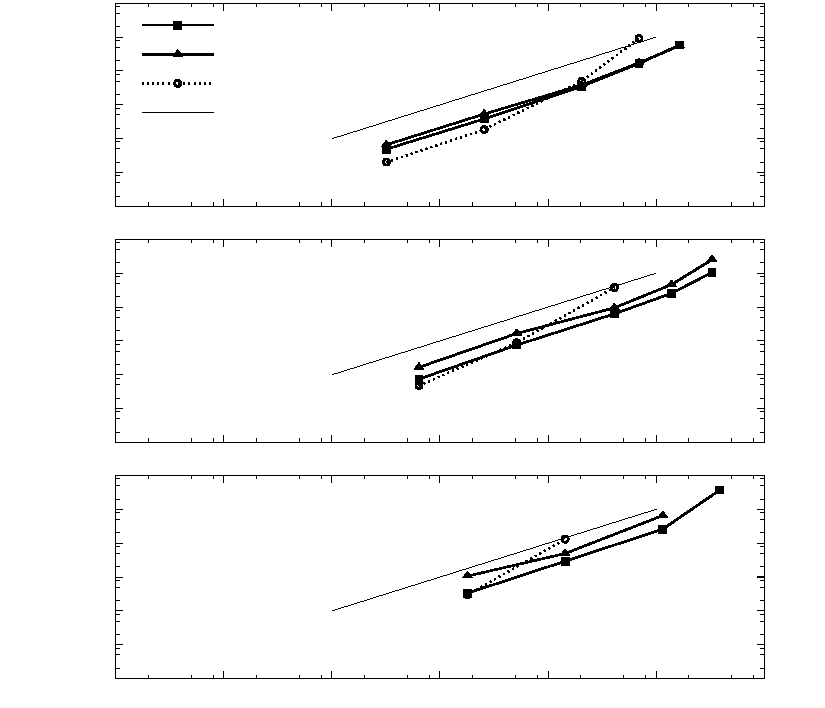
\includegraphics{ConstCoeffPoissonScaling}}%
    \gplfronttext
  \end{picture}%
\endgroup

\end{center}
\caption{
Solver runtime vs. degrees-of-freedom, for different polynomial degrees $k$,
for problem/Equation (\ref{eq:ContantCoeffPoissonBenchmark}).
}
\label{fig:ConstantCoeffRuntimes}
\end{figure}
\newpage
\section{Solver Performance - Navier-Stokes problems}
\label{sec:SolverPerformanceNSE}
Different solver strategies are conducted to solve the fully coupled incompressible Navier-Stokes equations. At the moment the following strategies can be examined:
\begin{itemize}
	\item Linearizsation of the NSE with: Newton(Gmres) or Picard
	\item Solving the linear problem with a Gmres approach or the direct solver MUMPS
	\item Preconditioning with Additive-Schwarz domain decomposition (with coarse solve on the coarsest multigrid level) and direct solver MUMPS for the Blocks (Automatic)
	\item Preconditioning with Additive-Schwarz kcycle Blocks on the coarsest multigrid level (with coarse solve on the coarsest multigrid level) and direct solver MUMPS for the Blocks
\end{itemize}
\subsection{Driven Cavity 3D}
The problem
\begin{equation}
\left\{ \begin{array} {rclll}
\rho_f\Big(\frac{\partial \vec{u}}{\partial t}+ \vec{u} \cdot \nabla \vec{u}\Big) +\nabla p - \mu_f \Delta \vec{u} & = & \vec{f}                   
& \text{and}\   &  \\
% ----
\nabla \cdot \vec{u} & = & 0                             
& \text{in}\ \Omega = (-0.5,0.5) \times (-0.5,0.5) \times (-0.5,0.5)  & \\
\vec{u}_D & = & \{1,0,0 \}                             
& \text{on}\ \Gamma_D = \{ (x,y,0z) \in \real^3; \ z = 0.5 \} 
& \text{Dirichlet-boundary}\\
\vec{u}_W & = & 0  
& \text{on}\ \Gamma_W = \partial \Omega \setminus \Gamma_D
& \text{Dirichlet-boundary}\\
\vec{u}_0(x,y,z) & = & \{1,0,0\}  
& \text{in}\ \Omega = (-0.5,0.5) \times (-0.5,0.5) \times (-0.5,0.5)  
& \text{Initial Condition}
\end{array} \right.
\label{eq:NavierStokesCavityBenchmark}
\end{equation}
is investigated on different cartesian grids. The physical parameters of the fluid are choosen to be $\rho_f=1$ and $\mu_f=0.0025$ which renders down to a Reynoldsnumber of 400.

\graphicspath{{./apdx-NodeSolverPerformance/NavierStokesDrivenCavity/plots/}}

\begin{figure}[h!]
	\begin{center}
		% GNUPLOT: LaTeX picture with Postscript
\begingroup
  \makeatletter
  \providecommand\color[2][]{%
    \GenericError{(gnuplot) \space\space\space\@spaces}{%
      Package color not loaded in conjunction with
      terminal option `colourtext'%
    }{See the gnuplot documentation for explanation.%
    }{Either use 'blacktext' in gnuplot or load the package
      color.sty in LaTeX.}%
    \renewcommand\color[2][]{}%
  }%
  \providecommand\includegraphics[2][]{%
    \GenericError{(gnuplot) \space\space\space\@spaces}{%
      Package graphicx or graphics not loaded%
    }{See the gnuplot documentation for explanation.%
    }{The gnuplot epslatex terminal needs graphicx.sty or graphics.sty.}%
    \renewcommand\includegraphics[2][]{}%
  }%
  \providecommand\rotatebox[2]{#2}%
  \@ifundefined{ifGPcolor}{%
    \newif\ifGPcolor
    \GPcolortrue
  }{}%
  \@ifundefined{ifGPblacktext}{%
    \newif\ifGPblacktext
    \GPblacktexttrue
  }{}%
  % define a \g@addto@macro without @ in the name:
  \let\gplgaddtomacro\g@addto@macro
  % define empty templates for all commands taking text:
  \gdef\gplbacktext{}%
  \gdef\gplfronttext{}%
  \makeatother
  \ifGPblacktext
    % no textcolor at all
    \def\colorrgb#1{}%
    \def\colorgray#1{}%
  \else
    % gray or color?
    \ifGPcolor
      \def\colorrgb#1{\color[rgb]{#1}}%
      \def\colorgray#1{\color[gray]{#1}}%
      \expandafter\def\csname LTw\endcsname{\color{white}}%
      \expandafter\def\csname LTb\endcsname{\color{black}}%
      \expandafter\def\csname LTa\endcsname{\color{black}}%
      \expandafter\def\csname LT0\endcsname{\color[rgb]{1,0,0}}%
      \expandafter\def\csname LT1\endcsname{\color[rgb]{0,1,0}}%
      \expandafter\def\csname LT2\endcsname{\color[rgb]{0,0,1}}%
      \expandafter\def\csname LT3\endcsname{\color[rgb]{1,0,1}}%
      \expandafter\def\csname LT4\endcsname{\color[rgb]{0,1,1}}%
      \expandafter\def\csname LT5\endcsname{\color[rgb]{1,1,0}}%
      \expandafter\def\csname LT6\endcsname{\color[rgb]{0,0,0}}%
      \expandafter\def\csname LT7\endcsname{\color[rgb]{1,0.3,0}}%
      \expandafter\def\csname LT8\endcsname{\color[rgb]{0.5,0.5,0.5}}%
    \else
      % gray
      \def\colorrgb#1{\color{black}}%
      \def\colorgray#1{\color[gray]{#1}}%
      \expandafter\def\csname LTw\endcsname{\color{white}}%
      \expandafter\def\csname LTb\endcsname{\color{black}}%
      \expandafter\def\csname LTa\endcsname{\color{black}}%
      \expandafter\def\csname LT0\endcsname{\color{black}}%
      \expandafter\def\csname LT1\endcsname{\color{black}}%
      \expandafter\def\csname LT2\endcsname{\color{black}}%
      \expandafter\def\csname LT3\endcsname{\color{black}}%
      \expandafter\def\csname LT4\endcsname{\color{black}}%
      \expandafter\def\csname LT5\endcsname{\color{black}}%
      \expandafter\def\csname LT6\endcsname{\color{black}}%
      \expandafter\def\csname LT7\endcsname{\color{black}}%
      \expandafter\def\csname LT8\endcsname{\color{black}}%
    \fi
  \fi
    \setlength{\unitlength}{0.0500bp}%
    \ifx\gptboxheight\undefined%
      \newlength{\gptboxheight}%
      \newlength{\gptboxwidth}%
      \newsavebox{\gptboxtext}%
    \fi%
    \setlength{\fboxrule}{0.5pt}%
    \setlength{\fboxsep}{1pt}%
\begin{picture}(12460.00,5660.00)%
    \gplgaddtomacro\gplbacktext{%
      \csname LTb\endcsname%
      \put(762,772){\makebox(0,0)[r]{\strut{}$10^{1}$}}%
      \csname LTb\endcsname%
      \put(762,1801){\makebox(0,0)[r]{\strut{}$10^{2}$}}%
      \csname LTb\endcsname%
      \put(762,2829){\makebox(0,0)[r]{\strut{}$10^{3}$}}%
      \csname LTb\endcsname%
      \put(762,3858){\makebox(0,0)[r]{\strut{}$10^{4}$}}%
      \csname LTb\endcsname%
      \put(762,4886){\makebox(0,0)[r]{\strut{}$10^{5}$}}%
      \csname LTb\endcsname%
      \put(864,593){\makebox(0,0){\strut{}$10^{3}$}}%
      \csname LTb\endcsname%
      \put(2420,593){\makebox(0,0){\strut{}$10^{4}$}}%
      \csname LTb\endcsname%
      \put(3975,593){\makebox(0,0){\strut{}$10^{5}$}}%
      \csname LTb\endcsname%
      \put(5531,593){\makebox(0,0){\strut{}$10^{6}$}}%
      \csname LTb\endcsname%
      \put(5633,772){\makebox(0,0)[l]{\strut{} }}%
      \csname LTb\endcsname%
      \put(5633,1286){\makebox(0,0)[l]{\strut{} }}%
      \csname LTb\endcsname%
      \put(5633,1801){\makebox(0,0)[l]{\strut{} }}%
      \csname LTb\endcsname%
      \put(5633,2315){\makebox(0,0)[l]{\strut{} }}%
      \csname LTb\endcsname%
      \put(5633,2829){\makebox(0,0)[l]{\strut{} }}%
      \csname LTb\endcsname%
      \put(5633,3343){\makebox(0,0)[l]{\strut{} }}%
      \csname LTb\endcsname%
      \put(5633,3858){\makebox(0,0)[l]{\strut{} }}%
      \csname LTb\endcsname%
      \put(5633,4372){\makebox(0,0)[l]{\strut{} }}%
      \csname LTb\endcsname%
      \put(5633,4886){\makebox(0,0)[l]{\strut{} }}%
      \csname LTb\endcsname%
      \put(864,5065){\makebox(0,0){\strut{} }}%
      \csname LTb\endcsname%
      \put(1531,5065){\makebox(0,0){\strut{} }}%
      \csname LTb\endcsname%
      \put(2197,5065){\makebox(0,0){\strut{} }}%
      \csname LTb\endcsname%
      \put(2864,5065){\makebox(0,0){\strut{} }}%
      \csname LTb\endcsname%
      \put(3531,5065){\makebox(0,0){\strut{} }}%
      \csname LTb\endcsname%
      \put(4198,5065){\makebox(0,0){\strut{} }}%
      \csname LTb\endcsname%
      \put(4864,5065){\makebox(0,0){\strut{} }}%
      \csname LTb\endcsname%
      \put(5531,5065){\makebox(0,0){\strut{} }}%
    }%
    \gplgaddtomacro\gplfronttext{%
      \csname LTb\endcsname%
      \put(264,2829){\rotatebox{-270}{\makebox(0,0){\strut{}Time [s]}}}%
      \csname LTb\endcsname%
      \put(3197,325){\makebox(0,0){\strut{}TotalDoFs}}%
      \csname LTb\endcsname%
      \put(11549,4796){\makebox(0,0)[r]{\strut{}Picard Mumps MGLevels1}}%
      \csname LTb\endcsname%
      \put(11549,4617){\makebox(0,0)[r]{\strut{}NewtonGmres Automatic MGLevels2}}%
      \csname LTb\endcsname%
      \put(11549,4438){\makebox(0,0)[r]{\strut{}NewtonGmres Mumps MGLevels1}}%
      \csname LTb\endcsname%
      \put(11549,4259){\makebox(0,0)[r]{\strut{}Newton Mumps MGLevels1}}%
      \csname LTb\endcsname%
      \put(11549,4080){\makebox(0,0)[r]{\strut{}NewtonGmres Swz Kcycle w Coarse Overlap MGLevels2}}%
      \csname LTb\endcsname%
      \put(11549,3901){\makebox(0,0)[r]{\strut{}Picard SoftGMRES Swz Kcycle w Coarse Overlap MGLevels2}}%
    }%
    \gplbacktext
    \put(0,0){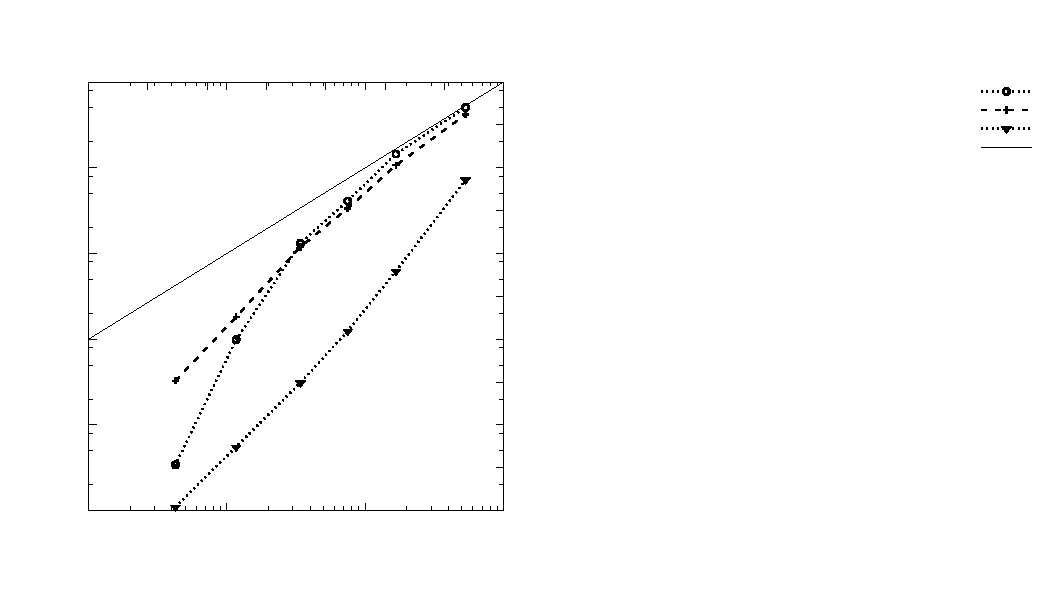
\includegraphics{NodePerformance}}%
    \gplfronttext
  \end{picture}%
\endgroup

	\end{center}
	\caption{
		Solver runtime vs. DoFs, for polynomial degree $k=2/1$,
		for problem/Equation (\ref{eq:NavierStokesCavityBenchmark}).
	}
	\label{fig:DrivenCavity}
\end{figure}


% ################################################################################
\chapter{Parallel Performance and Scaling}
\label{sec:ParallelPerformance}
% ################################################################################
This section covers basic performance tests, i.e. how specific algorithms scale in parallel with increasing \emph{number of processors}. So far, all calculations for this research were conducted on the Lichtenberg high performance computer of the TU Darmstadt

\section{Parallel Efficiency - Navier-Stokes problems}
Different solver strategies are conducted to solve the fully coupled incompressible Navier-Stokes equations. At the moment the following strategies can be examined:
\begin{itemize}
	\item Linearizsation of the NSE with: Newton(Gmres) or Picard
	\item Solving the linear problem with a Gmres approach
	\item Preconditioning with Additive-Schwarz domain decomposition (with coarse solve on the coarsest multigrid level) and direct solver MUMPS for the Blocks
\end{itemize}
\subsection{Simple 3D sphere immersed in a fluid flow}
\label{sec:MPIPerformanceSphere}
The problem
\begin{equation}
\left\{ \begin{array} {rclll}
\rho_f\Big(\frac{\partial \vec{u}}{\partial t}+ \vec{u} \cdot \nabla \vec{u}\Big) +\nabla p - \mu_f \Delta \vec{u} & = & \vec{f}                   
& \text{and}\   &  \\
% ----
\nabla \cdot \vec{u} & = & 0                             
& \text{in}\ \Omega = (-5,10) \times (-5,5) \times (-5,5)  & \\
 \vec{u}_D & = & 0                             
& \text{on}\ \Gamma_D = \{ (x,y,z,t) \in \real^3; \ z = -5,5 \} 
& \text{Dirichlet-boundary}\\
 \vec{u}_S & = & 0                             
 & \text{on}\ \Gamma_S = \{ (x,y,z) \in \real^3; \ x^2+y^2+z^2 = 1 \}
& \text{Dirichlet-boundary} \\
 p_O & = & 0                             
& \text{on}\ \Gamma_O = \{ (x,y,z) \in \real^3; \ x = 10 \}
& \text{Dirichlet-boundary} \\
% ----
\vec{u}(x,-5,z) & = & \vec{u}(x,5,z)  
& \text{on}\ \Gamma_P = \partial \Omega \setminus \Gamma_D \setminus \Gamma_S \setminus \Gamma_O
& \text{Periodic-boundary}\\
\vec{u}_0(x,y,z) & = & \{1,0,0\}  
& \text{in}\ \Omega = (-5,10) \times (-5,5) \times (-5,5)   
& \text{Initial Condition}
\end{array} \right.
\label{eq:NavierStokesSphereBenchmark}
\end{equation}
is investigated on a 64x16x16 cell Cartesian grid. The physical parameters of the fluid are choosen to be $\rho_f=1$ and $\mu_f=0.002$ which renders down to a Reynoldsnumber of 100. The problem basically describes a sphere flow between two plates.

\graphicspath{{./apdx-MPISolverPerformance/strongScaling/NSESphere/plots/}}

\begin{figure}[h!]
	\begin{center}
		% GNUPLOT: LaTeX picture with Postscript
\begingroup
  \makeatletter
  \providecommand\color[2][]{%
    \GenericError{(gnuplot) \space\space\space\@spaces}{%
      Package color not loaded in conjunction with
      terminal option `colourtext'%
    }{See the gnuplot documentation for explanation.%
    }{Either use 'blacktext' in gnuplot or load the package
      color.sty in LaTeX.}%
    \renewcommand\color[2][]{}%
  }%
  \providecommand\includegraphics[2][]{%
    \GenericError{(gnuplot) \space\space\space\@spaces}{%
      Package graphicx or graphics not loaded%
    }{See the gnuplot documentation for explanation.%
    }{The gnuplot epslatex terminal needs graphicx.sty or graphics.sty.}%
    \renewcommand\includegraphics[2][]{}%
  }%
  \providecommand\rotatebox[2]{#2}%
  \@ifundefined{ifGPcolor}{%
    \newif\ifGPcolor
    \GPcolortrue
  }{}%
  \@ifundefined{ifGPblacktext}{%
    \newif\ifGPblacktext
    \GPblacktexttrue
  }{}%
  % define a \g@addto@macro without @ in the name:
  \let\gplgaddtomacro\g@addto@macro
  % define empty templates for all commands taking text:
  \gdef\gplbacktext{}%
  \gdef\gplfronttext{}%
  \makeatother
  \ifGPblacktext
    % no textcolor at all
    \def\colorrgb#1{}%
    \def\colorgray#1{}%
  \else
    % gray or color?
    \ifGPcolor
      \def\colorrgb#1{\color[rgb]{#1}}%
      \def\colorgray#1{\color[gray]{#1}}%
      \expandafter\def\csname LTw\endcsname{\color{white}}%
      \expandafter\def\csname LTb\endcsname{\color{black}}%
      \expandafter\def\csname LTa\endcsname{\color{black}}%
      \expandafter\def\csname LT0\endcsname{\color[rgb]{1,0,0}}%
      \expandafter\def\csname LT1\endcsname{\color[rgb]{0,1,0}}%
      \expandafter\def\csname LT2\endcsname{\color[rgb]{0,0,1}}%
      \expandafter\def\csname LT3\endcsname{\color[rgb]{1,0,1}}%
      \expandafter\def\csname LT4\endcsname{\color[rgb]{0,1,1}}%
      \expandafter\def\csname LT5\endcsname{\color[rgb]{1,1,0}}%
      \expandafter\def\csname LT6\endcsname{\color[rgb]{0,0,0}}%
      \expandafter\def\csname LT7\endcsname{\color[rgb]{1,0.3,0}}%
      \expandafter\def\csname LT8\endcsname{\color[rgb]{0.5,0.5,0.5}}%
    \else
      % gray
      \def\colorrgb#1{\color{black}}%
      \def\colorgray#1{\color[gray]{#1}}%
      \expandafter\def\csname LTw\endcsname{\color{white}}%
      \expandafter\def\csname LTb\endcsname{\color{black}}%
      \expandafter\def\csname LTa\endcsname{\color{black}}%
      \expandafter\def\csname LT0\endcsname{\color{black}}%
      \expandafter\def\csname LT1\endcsname{\color{black}}%
      \expandafter\def\csname LT2\endcsname{\color{black}}%
      \expandafter\def\csname LT3\endcsname{\color{black}}%
      \expandafter\def\csname LT4\endcsname{\color{black}}%
      \expandafter\def\csname LT5\endcsname{\color{black}}%
      \expandafter\def\csname LT6\endcsname{\color{black}}%
      \expandafter\def\csname LT7\endcsname{\color{black}}%
      \expandafter\def\csname LT8\endcsname{\color{black}}%
    \fi
  \fi
    \setlength{\unitlength}{0.0500bp}%
    \ifx\gptboxheight\undefined%
      \newlength{\gptboxheight}%
      \newlength{\gptboxwidth}%
      \newsavebox{\gptboxtext}%
    \fi%
    \setlength{\fboxrule}{0.5pt}%
    \setlength{\fboxsep}{1pt}%
\begin{picture}(9620.00,9620.00)%
    \gplgaddtomacro\gplbacktext{%
      \csname LTb\endcsname%
      \put(691,5057){\makebox(0,0)[r]{\strut{}$150$}}%
      \csname LTb\endcsname%
      \put(691,5429){\makebox(0,0)[r]{\strut{}$200$}}%
      \csname LTb\endcsname%
      \put(691,5801){\makebox(0,0)[r]{\strut{}$250$}}%
      \csname LTb\endcsname%
      \put(691,6172){\makebox(0,0)[r]{\strut{}$300$}}%
      \csname LTb\endcsname%
      \put(691,6544){\makebox(0,0)[r]{\strut{}$350$}}%
      \csname LTb\endcsname%
      \put(691,6916){\makebox(0,0)[r]{\strut{}$400$}}%
      \csname LTb\endcsname%
      \put(691,7288){\makebox(0,0)[r]{\strut{}$450$}}%
      \csname LTb\endcsname%
      \put(691,7660){\makebox(0,0)[r]{\strut{}$500$}}%
      \csname LTb\endcsname%
      \put(691,8031){\makebox(0,0)[r]{\strut{}$550$}}%
      \csname LTb\endcsname%
      \put(691,8403){\makebox(0,0)[r]{\strut{}$600$}}%
      \csname LTb\endcsname%
      \put(691,8775){\makebox(0,0)[r]{\strut{}$650$}}%
      \csname LTb\endcsname%
      \put(1335,4858){\makebox(0,0){\strut{}$10$}}%
      \csname LTb\endcsname%
      \put(1952,4858){\makebox(0,0){\strut{}$20$}}%
      \csname LTb\endcsname%
      \put(2569,4858){\makebox(0,0){\strut{}$30$}}%
      \csname LTb\endcsname%
      \put(3186,4858){\makebox(0,0){\strut{}$40$}}%
      \csname LTb\endcsname%
      \put(3804,4858){\makebox(0,0){\strut{}$50$}}%
      \csname LTb\endcsname%
      \put(4421,4858){\makebox(0,0){\strut{}$60$}}%
      \csname LTb\endcsname%
      \put(4756,5057){\makebox(0,0)[l]{\strut{} }}%
      \csname LTb\endcsname%
      \put(4756,5429){\makebox(0,0)[l]{\strut{} }}%
      \csname LTb\endcsname%
      \put(4756,5801){\makebox(0,0)[l]{\strut{} }}%
      \csname LTb\endcsname%
      \put(4756,6172){\makebox(0,0)[l]{\strut{} }}%
      \csname LTb\endcsname%
      \put(4756,6544){\makebox(0,0)[l]{\strut{} }}%
      \csname LTb\endcsname%
      \put(4756,6916){\makebox(0,0)[l]{\strut{} }}%
      \csname LTb\endcsname%
      \put(4756,7288){\makebox(0,0)[l]{\strut{} }}%
      \csname LTb\endcsname%
      \put(4756,7660){\makebox(0,0)[l]{\strut{} }}%
      \csname LTb\endcsname%
      \put(4756,8031){\makebox(0,0)[l]{\strut{} }}%
      \csname LTb\endcsname%
      \put(4756,8403){\makebox(0,0)[l]{\strut{} }}%
      \csname LTb\endcsname%
      \put(4756,8775){\makebox(0,0)[l]{\strut{} }}%
      \csname LTb\endcsname%
      \put(779,8974){\makebox(0,0){\strut{} }}%
      \csname LTb\endcsname%
      \put(1335,8974){\makebox(0,0){\strut{} }}%
      \csname LTb\endcsname%
      \put(1890,8974){\makebox(0,0){\strut{} }}%
      \csname LTb\endcsname%
      \put(2446,8974){\makebox(0,0){\strut{} }}%
      \csname LTb\endcsname%
      \put(3001,8974){\makebox(0,0){\strut{} }}%
      \csname LTb\endcsname%
      \put(3557,8974){\makebox(0,0){\strut{} }}%
      \csname LTb\endcsname%
      \put(4112,8974){\makebox(0,0){\strut{} }}%
      \csname LTb\endcsname%
      \put(4668,8974){\makebox(0,0){\strut{} }}%
    }%
    \gplgaddtomacro\gplfronttext{%
      \csname LTb\endcsname%
      \put(239,6916){\rotatebox{-270}{\makebox(0,0){\strut{}Time [s]}}}%
      \csname LTb\endcsname%
      \put(5030,6916){\rotatebox{-270}{\makebox(0,0){\strut{}SlvIter}}}%
      \csname LTb\endcsname%
      \put(2723,9472){\makebox(0,0){\strut{}Exclusive times}}%
      \csname LTb\endcsname%
      \put(8827,8675){\makebox(0,0)[r]{\strut{}Automatic MGLevels3}}%
      \csname LTb\endcsname%
      \put(8827,8476){\makebox(0,0)[r]{\strut{}SoftGMRES Swz w Coarse Overlap MGLevels3}}%
    }%
    \gplgaddtomacro\gplbacktext{%
      \csname LTb\endcsname%
      \put(691,684){\makebox(0,0)[r]{\strut{}$0.5$}}%
      \csname LTb\endcsname%
      \put(691,1169){\makebox(0,0)[r]{\strut{}$1$}}%
      \csname LTb\endcsname%
      \put(691,1654){\makebox(0,0)[r]{\strut{}$1.5$}}%
      \csname LTb\endcsname%
      \put(691,2138){\makebox(0,0)[r]{\strut{}$2$}}%
      \csname LTb\endcsname%
      \put(691,2623){\makebox(0,0)[r]{\strut{}$2.5$}}%
      \csname LTb\endcsname%
      \put(691,3108){\makebox(0,0)[r]{\strut{}$3$}}%
      \csname LTb\endcsname%
      \put(691,3593){\makebox(0,0)[r]{\strut{}$3.5$}}%
      \csname LTb\endcsname%
      \put(691,4077){\makebox(0,0)[r]{\strut{}$4$}}%
      \csname LTb\endcsname%
      \put(691,4562){\makebox(0,0)[r]{\strut{}$4.5$}}%
      \csname LTb\endcsname%
      \put(1335,485){\makebox(0,0){\strut{}$10$}}%
      \csname LTb\endcsname%
      \put(1952,485){\makebox(0,0){\strut{}$20$}}%
      \csname LTb\endcsname%
      \put(2569,485){\makebox(0,0){\strut{}$30$}}%
      \csname LTb\endcsname%
      \put(3186,485){\makebox(0,0){\strut{}$40$}}%
      \csname LTb\endcsname%
      \put(3804,485){\makebox(0,0){\strut{}$50$}}%
      \csname LTb\endcsname%
      \put(4421,485){\makebox(0,0){\strut{}$60$}}%
      \csname LTb\endcsname%
      \put(4756,684){\makebox(0,0)[l]{\strut{} }}%
      \csname LTb\endcsname%
      \put(4756,1169){\makebox(0,0)[l]{\strut{} }}%
      \csname LTb\endcsname%
      \put(4756,1654){\makebox(0,0)[l]{\strut{} }}%
      \csname LTb\endcsname%
      \put(4756,2138){\makebox(0,0)[l]{\strut{} }}%
      \csname LTb\endcsname%
      \put(4756,2623){\makebox(0,0)[l]{\strut{} }}%
      \csname LTb\endcsname%
      \put(4756,3108){\makebox(0,0)[l]{\strut{} }}%
      \csname LTb\endcsname%
      \put(4756,3593){\makebox(0,0)[l]{\strut{} }}%
      \csname LTb\endcsname%
      \put(4756,4077){\makebox(0,0)[l]{\strut{} }}%
      \csname LTb\endcsname%
      \put(4756,4562){\makebox(0,0)[l]{\strut{} }}%
      \csname LTb\endcsname%
      \put(779,4761){\makebox(0,0){\strut{} }}%
      \csname LTb\endcsname%
      \put(1335,4761){\makebox(0,0){\strut{} }}%
      \csname LTb\endcsname%
      \put(1890,4761){\makebox(0,0){\strut{} }}%
      \csname LTb\endcsname%
      \put(2446,4761){\makebox(0,0){\strut{} }}%
      \csname LTb\endcsname%
      \put(3001,4761){\makebox(0,0){\strut{} }}%
      \csname LTb\endcsname%
      \put(3557,4761){\makebox(0,0){\strut{} }}%
      \csname LTb\endcsname%
      \put(4112,4761){\makebox(0,0){\strut{} }}%
      \csname LTb\endcsname%
      \put(4668,4761){\makebox(0,0){\strut{} }}%
    }%
    \gplgaddtomacro\gplfronttext{%
      \csname LTb\endcsname%
      \put(239,2623){\rotatebox{-270}{\makebox(0,0){\strut{}Time [s]}}}%
      \csname LTb\endcsname%
      \put(5030,2623){\rotatebox{-270}{\makebox(0,0){\strut{}SlvInit}}}%
      \csname LTb\endcsname%
      \put(2723,187){\makebox(0,0){\strut{}Processors}}%
      \csname LTb\endcsname%
      \put(8827,4462){\makebox(0,0)[r]{\strut{}Automatic MGLevels3}}%
      \csname LTb\endcsname%
      \put(8827,4263){\makebox(0,0)[r]{\strut{}SoftGMRES Swz w Coarse Overlap MGLevels3}}%
    }%
    \gplbacktext
    \put(0,0){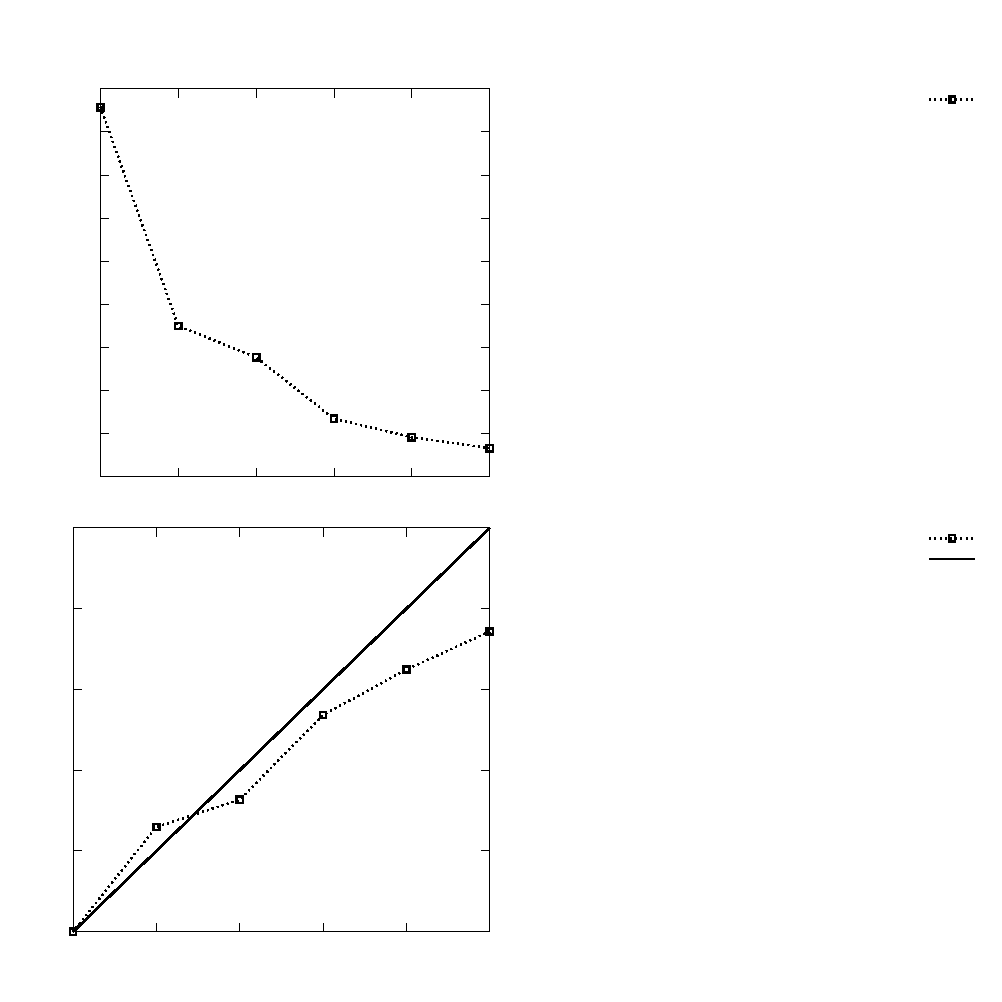
\includegraphics{MPIScalingTimes}}%
    \gplfronttext
  \end{picture}%
\endgroup

	\end{center}
	\caption{
		Solver runtime vs. processors, for polynomial degree $k=1/0$ leading to 212992 DoFs,
		for problem/Equation (\ref{eq:ContantCoeffPoissonBenchmark}).
	}
	\label{fig:Spherek1Time}
\end{figure}

\graphicspath{{./apdx-MPISolverPerformance/strongScaling/NSESphereComplex/plots/}}

\begin{figure}[h!]
	\begin{center}
		% GNUPLOT: LaTeX picture with Postscript
\begingroup
  \makeatletter
  \providecommand\color[2][]{%
    \GenericError{(gnuplot) \space\space\space\@spaces}{%
      Package color not loaded in conjunction with
      terminal option `colourtext'%
    }{See the gnuplot documentation for explanation.%
    }{Either use 'blacktext' in gnuplot or load the package
      color.sty in LaTeX.}%
    \renewcommand\color[2][]{}%
  }%
  \providecommand\includegraphics[2][]{%
    \GenericError{(gnuplot) \space\space\space\@spaces}{%
      Package graphicx or graphics not loaded%
    }{See the gnuplot documentation for explanation.%
    }{The gnuplot epslatex terminal needs graphicx.sty or graphics.sty.}%
    \renewcommand\includegraphics[2][]{}%
  }%
  \providecommand\rotatebox[2]{#2}%
  \@ifundefined{ifGPcolor}{%
    \newif\ifGPcolor
    \GPcolortrue
  }{}%
  \@ifundefined{ifGPblacktext}{%
    \newif\ifGPblacktext
    \GPblacktexttrue
  }{}%
  % define a \g@addto@macro without @ in the name:
  \let\gplgaddtomacro\g@addto@macro
  % define empty templates for all commands taking text:
  \gdef\gplbacktext{}%
  \gdef\gplfronttext{}%
  \makeatother
  \ifGPblacktext
    % no textcolor at all
    \def\colorrgb#1{}%
    \def\colorgray#1{}%
  \else
    % gray or color?
    \ifGPcolor
      \def\colorrgb#1{\color[rgb]{#1}}%
      \def\colorgray#1{\color[gray]{#1}}%
      \expandafter\def\csname LTw\endcsname{\color{white}}%
      \expandafter\def\csname LTb\endcsname{\color{black}}%
      \expandafter\def\csname LTa\endcsname{\color{black}}%
      \expandafter\def\csname LT0\endcsname{\color[rgb]{1,0,0}}%
      \expandafter\def\csname LT1\endcsname{\color[rgb]{0,1,0}}%
      \expandafter\def\csname LT2\endcsname{\color[rgb]{0,0,1}}%
      \expandafter\def\csname LT3\endcsname{\color[rgb]{1,0,1}}%
      \expandafter\def\csname LT4\endcsname{\color[rgb]{0,1,1}}%
      \expandafter\def\csname LT5\endcsname{\color[rgb]{1,1,0}}%
      \expandafter\def\csname LT6\endcsname{\color[rgb]{0,0,0}}%
      \expandafter\def\csname LT7\endcsname{\color[rgb]{1,0.3,0}}%
      \expandafter\def\csname LT8\endcsname{\color[rgb]{0.5,0.5,0.5}}%
    \else
      % gray
      \def\colorrgb#1{\color{black}}%
      \def\colorgray#1{\color[gray]{#1}}%
      \expandafter\def\csname LTw\endcsname{\color{white}}%
      \expandafter\def\csname LTb\endcsname{\color{black}}%
      \expandafter\def\csname LTa\endcsname{\color{black}}%
      \expandafter\def\csname LT0\endcsname{\color{black}}%
      \expandafter\def\csname LT1\endcsname{\color{black}}%
      \expandafter\def\csname LT2\endcsname{\color{black}}%
      \expandafter\def\csname LT3\endcsname{\color{black}}%
      \expandafter\def\csname LT4\endcsname{\color{black}}%
      \expandafter\def\csname LT5\endcsname{\color{black}}%
      \expandafter\def\csname LT6\endcsname{\color{black}}%
      \expandafter\def\csname LT7\endcsname{\color{black}}%
      \expandafter\def\csname LT8\endcsname{\color{black}}%
    \fi
  \fi
    \setlength{\unitlength}{0.0500bp}%
    \ifx\gptboxheight\undefined%
      \newlength{\gptboxheight}%
      \newlength{\gptboxwidth}%
      \newsavebox{\gptboxtext}%
    \fi%
    \setlength{\fboxrule}{0.5pt}%
    \setlength{\fboxsep}{1pt}%
\begin{picture}(9620.00,9620.00)%
    \gplgaddtomacro\gplbacktext{%
      \csname LTb\endcsname%
      \put(691,5057){\makebox(0,0)[r]{\strut{}$150$}}%
      \csname LTb\endcsname%
      \put(691,5429){\makebox(0,0)[r]{\strut{}$200$}}%
      \csname LTb\endcsname%
      \put(691,5801){\makebox(0,0)[r]{\strut{}$250$}}%
      \csname LTb\endcsname%
      \put(691,6172){\makebox(0,0)[r]{\strut{}$300$}}%
      \csname LTb\endcsname%
      \put(691,6544){\makebox(0,0)[r]{\strut{}$350$}}%
      \csname LTb\endcsname%
      \put(691,6916){\makebox(0,0)[r]{\strut{}$400$}}%
      \csname LTb\endcsname%
      \put(691,7288){\makebox(0,0)[r]{\strut{}$450$}}%
      \csname LTb\endcsname%
      \put(691,7660){\makebox(0,0)[r]{\strut{}$500$}}%
      \csname LTb\endcsname%
      \put(691,8031){\makebox(0,0)[r]{\strut{}$550$}}%
      \csname LTb\endcsname%
      \put(691,8403){\makebox(0,0)[r]{\strut{}$600$}}%
      \csname LTb\endcsname%
      \put(691,8775){\makebox(0,0)[r]{\strut{}$650$}}%
      \csname LTb\endcsname%
      \put(1335,4858){\makebox(0,0){\strut{}$10$}}%
      \csname LTb\endcsname%
      \put(1952,4858){\makebox(0,0){\strut{}$20$}}%
      \csname LTb\endcsname%
      \put(2569,4858){\makebox(0,0){\strut{}$30$}}%
      \csname LTb\endcsname%
      \put(3186,4858){\makebox(0,0){\strut{}$40$}}%
      \csname LTb\endcsname%
      \put(3804,4858){\makebox(0,0){\strut{}$50$}}%
      \csname LTb\endcsname%
      \put(4421,4858){\makebox(0,0){\strut{}$60$}}%
      \csname LTb\endcsname%
      \put(4756,5057){\makebox(0,0)[l]{\strut{} }}%
      \csname LTb\endcsname%
      \put(4756,5429){\makebox(0,0)[l]{\strut{} }}%
      \csname LTb\endcsname%
      \put(4756,5801){\makebox(0,0)[l]{\strut{} }}%
      \csname LTb\endcsname%
      \put(4756,6172){\makebox(0,0)[l]{\strut{} }}%
      \csname LTb\endcsname%
      \put(4756,6544){\makebox(0,0)[l]{\strut{} }}%
      \csname LTb\endcsname%
      \put(4756,6916){\makebox(0,0)[l]{\strut{} }}%
      \csname LTb\endcsname%
      \put(4756,7288){\makebox(0,0)[l]{\strut{} }}%
      \csname LTb\endcsname%
      \put(4756,7660){\makebox(0,0)[l]{\strut{} }}%
      \csname LTb\endcsname%
      \put(4756,8031){\makebox(0,0)[l]{\strut{} }}%
      \csname LTb\endcsname%
      \put(4756,8403){\makebox(0,0)[l]{\strut{} }}%
      \csname LTb\endcsname%
      \put(4756,8775){\makebox(0,0)[l]{\strut{} }}%
      \csname LTb\endcsname%
      \put(779,8974){\makebox(0,0){\strut{} }}%
      \csname LTb\endcsname%
      \put(1335,8974){\makebox(0,0){\strut{} }}%
      \csname LTb\endcsname%
      \put(1890,8974){\makebox(0,0){\strut{} }}%
      \csname LTb\endcsname%
      \put(2446,8974){\makebox(0,0){\strut{} }}%
      \csname LTb\endcsname%
      \put(3001,8974){\makebox(0,0){\strut{} }}%
      \csname LTb\endcsname%
      \put(3557,8974){\makebox(0,0){\strut{} }}%
      \csname LTb\endcsname%
      \put(4112,8974){\makebox(0,0){\strut{} }}%
      \csname LTb\endcsname%
      \put(4668,8974){\makebox(0,0){\strut{} }}%
    }%
    \gplgaddtomacro\gplfronttext{%
      \csname LTb\endcsname%
      \put(239,6916){\rotatebox{-270}{\makebox(0,0){\strut{}Time [s]}}}%
      \csname LTb\endcsname%
      \put(5030,6916){\rotatebox{-270}{\makebox(0,0){\strut{}SlvIter}}}%
      \csname LTb\endcsname%
      \put(2723,9472){\makebox(0,0){\strut{}Exclusive times}}%
      \csname LTb\endcsname%
      \put(8827,8675){\makebox(0,0)[r]{\strut{}Automatic MGLevels3}}%
      \csname LTb\endcsname%
      \put(8827,8476){\makebox(0,0)[r]{\strut{}SoftGMRES Swz w Coarse Overlap MGLevels3}}%
    }%
    \gplgaddtomacro\gplbacktext{%
      \csname LTb\endcsname%
      \put(691,684){\makebox(0,0)[r]{\strut{}$0.5$}}%
      \csname LTb\endcsname%
      \put(691,1169){\makebox(0,0)[r]{\strut{}$1$}}%
      \csname LTb\endcsname%
      \put(691,1654){\makebox(0,0)[r]{\strut{}$1.5$}}%
      \csname LTb\endcsname%
      \put(691,2138){\makebox(0,0)[r]{\strut{}$2$}}%
      \csname LTb\endcsname%
      \put(691,2623){\makebox(0,0)[r]{\strut{}$2.5$}}%
      \csname LTb\endcsname%
      \put(691,3108){\makebox(0,0)[r]{\strut{}$3$}}%
      \csname LTb\endcsname%
      \put(691,3593){\makebox(0,0)[r]{\strut{}$3.5$}}%
      \csname LTb\endcsname%
      \put(691,4077){\makebox(0,0)[r]{\strut{}$4$}}%
      \csname LTb\endcsname%
      \put(691,4562){\makebox(0,0)[r]{\strut{}$4.5$}}%
      \csname LTb\endcsname%
      \put(1335,485){\makebox(0,0){\strut{}$10$}}%
      \csname LTb\endcsname%
      \put(1952,485){\makebox(0,0){\strut{}$20$}}%
      \csname LTb\endcsname%
      \put(2569,485){\makebox(0,0){\strut{}$30$}}%
      \csname LTb\endcsname%
      \put(3186,485){\makebox(0,0){\strut{}$40$}}%
      \csname LTb\endcsname%
      \put(3804,485){\makebox(0,0){\strut{}$50$}}%
      \csname LTb\endcsname%
      \put(4421,485){\makebox(0,0){\strut{}$60$}}%
      \csname LTb\endcsname%
      \put(4756,684){\makebox(0,0)[l]{\strut{} }}%
      \csname LTb\endcsname%
      \put(4756,1169){\makebox(0,0)[l]{\strut{} }}%
      \csname LTb\endcsname%
      \put(4756,1654){\makebox(0,0)[l]{\strut{} }}%
      \csname LTb\endcsname%
      \put(4756,2138){\makebox(0,0)[l]{\strut{} }}%
      \csname LTb\endcsname%
      \put(4756,2623){\makebox(0,0)[l]{\strut{} }}%
      \csname LTb\endcsname%
      \put(4756,3108){\makebox(0,0)[l]{\strut{} }}%
      \csname LTb\endcsname%
      \put(4756,3593){\makebox(0,0)[l]{\strut{} }}%
      \csname LTb\endcsname%
      \put(4756,4077){\makebox(0,0)[l]{\strut{} }}%
      \csname LTb\endcsname%
      \put(4756,4562){\makebox(0,0)[l]{\strut{} }}%
      \csname LTb\endcsname%
      \put(779,4761){\makebox(0,0){\strut{} }}%
      \csname LTb\endcsname%
      \put(1335,4761){\makebox(0,0){\strut{} }}%
      \csname LTb\endcsname%
      \put(1890,4761){\makebox(0,0){\strut{} }}%
      \csname LTb\endcsname%
      \put(2446,4761){\makebox(0,0){\strut{} }}%
      \csname LTb\endcsname%
      \put(3001,4761){\makebox(0,0){\strut{} }}%
      \csname LTb\endcsname%
      \put(3557,4761){\makebox(0,0){\strut{} }}%
      \csname LTb\endcsname%
      \put(4112,4761){\makebox(0,0){\strut{} }}%
      \csname LTb\endcsname%
      \put(4668,4761){\makebox(0,0){\strut{} }}%
    }%
    \gplgaddtomacro\gplfronttext{%
      \csname LTb\endcsname%
      \put(239,2623){\rotatebox{-270}{\makebox(0,0){\strut{}Time [s]}}}%
      \csname LTb\endcsname%
      \put(5030,2623){\rotatebox{-270}{\makebox(0,0){\strut{}SlvInit}}}%
      \csname LTb\endcsname%
      \put(2723,187){\makebox(0,0){\strut{}Processors}}%
      \csname LTb\endcsname%
      \put(8827,4462){\makebox(0,0)[r]{\strut{}Automatic MGLevels3}}%
      \csname LTb\endcsname%
      \put(8827,4263){\makebox(0,0)[r]{\strut{}SoftGMRES Swz w Coarse Overlap MGLevels3}}%
    }%
    \gplbacktext
    \put(0,0){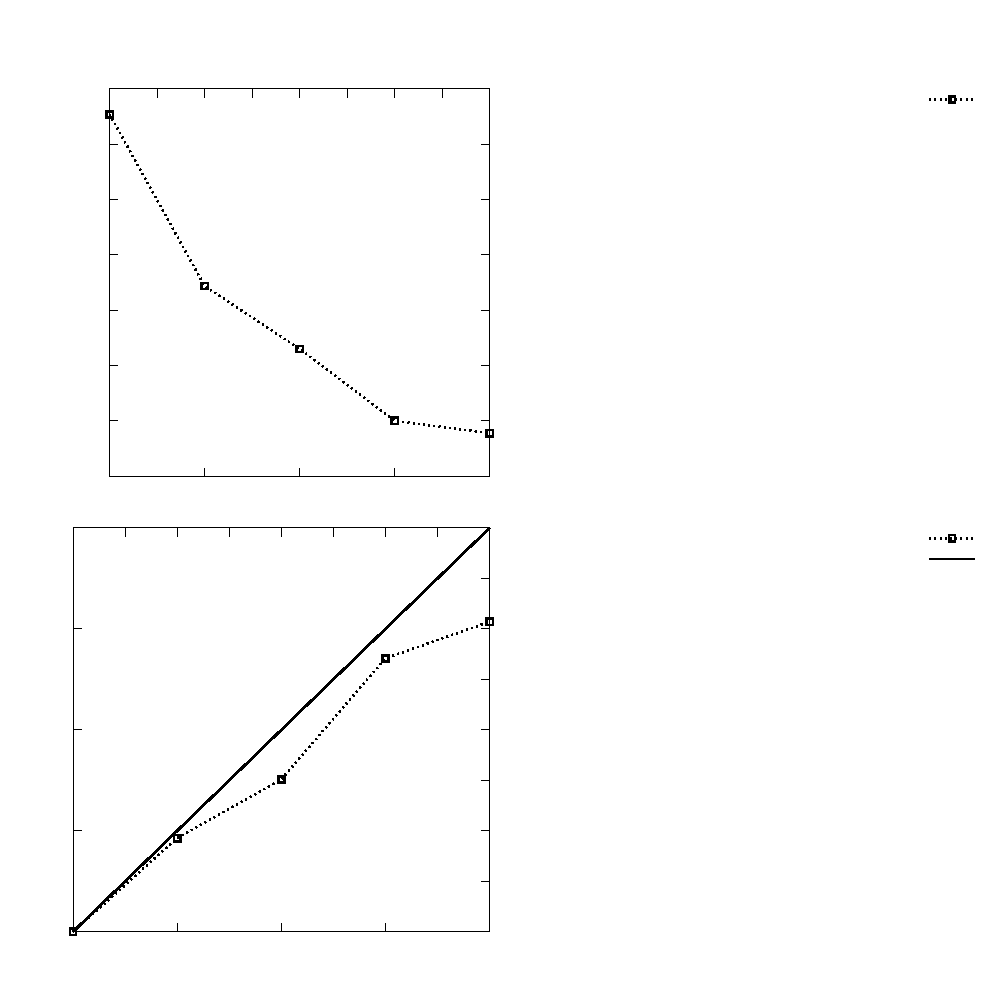
\includegraphics{MPIScalingTimes}}%
    \gplfronttext
  \end{picture}%
\endgroup

	\end{center}
	\caption{
		Solver runtime vs. processors, for polynomial degree $k=2/1$ leading to 557056 DoFs,
		for problem/Equation (\ref{eq:ContantCoeffPoissonBenchmark}).
	}
	\label{fig:Spherek1Time}
\end{figure}

\clearpage
\section{Weak Scaling - Navier-Stokes problems}
in progress...

% ################################################################################
\chapter{BoSSSpad command reference}
\label{sec:BoSSSpadReference}
% ################################################################################

% Change some settings so reference looks nice
\renewcommand{\ttdefault}{pcr} % Using Courier, so we can have bold typewriter font
\setdescription{
	font=\ttfamily\small\bfseries,
	labelindent=1em,
	leftmargin=.2\textwidth,
	style=nextline}

\section{Command line basics}

The command line uses C\# syntax.
On startup, the variable \lstinline{IList<IDatabaseInfo> databases} stores a list of all loaded databases. They can be accessed and modified by \BoSSSpad{}.

For most variables, the method \lstinline{Actions()} will display a (in rare situations, potentially incomplete) list of methods that are available.
\begin{lstlisting}
> databases.Actions()

You can invoke the following methods (more actions may exist):
- Actions()
- As()
- Cast()
- Actions(Boolean showBuiltinMethods)
- Describe()
- Describe(String methodName)
- Summary()
\end{lstlisting}

The most important methods are described in this document, but if you want to learn more about a particular method you can always use \lstinline{Describe("nameOfSomeMethod")} to get the full documentation from the source code.
\begin{lstlisting}
> databases.First().Sessions.Describe("Find")

ISessionInfo Find(PartialGuid guid):
   * Summary: Returns the single session that matches the given guid .
   * guid: The guid of session the session in question.
   * Returns: A single session that matches guid , if it exists. Otherwise,
     an error will be thrown.
\end{lstlisting}

Other useful commands are:
\begin{description}
	\item[Clear()]
	Clears the console window
	
	\item[ShowVars()]
	Displays all the variables that have been created during the \BoSSSpad{} session.

	\item[OpenConfigFile()]
	Opens the \lstinline{DBE.xml} with the default viewer for text files.
	
	\item[OpenConfigDirectory()]
	Opens an Explorer window of the folder containing the \lstinline{DBE.xml}, the \lstinline{DBErc.cs} and another configuration files.
	
	\item[LastError]
	Displays details concerning the last \lstinline{Exception} that occurred.
	
	\item[LoadAssembly(string pathToAssembly)]
	Loads the specified assembly into memory. Useful for loading assemblies that are not loaded by BoSSSPad by default.

	\item[SaveSessionAsWorksheet(string path)]
	Saves all commands with their respective results in the format ".bws" format than can be read by \BoSSSpad{}.
\end{description}

\subsection{Navigating through history}
\BoSSSpad{} maintains a history of the last 500 issued commands. The individual entries can be accessed in the style of the standard Unix/Linux shell \lstinline{Bash}. That is, commands can be accessed in the order of their submission using the up and down keys. Moreover, the page up and page down keys can be used to \emph{search} the history for commands that are equal to the current command up the current cursor position. As an example, consider the following command:
\begin{lstlisting}[title=Example history search]
databases.First().Sessions.Newest()
\end{lstlisting}
If the cursor position is at the end of the line, hitting the page up key will search the history for the last command that started with \lstinline{databases.First().Sessions.Newest()}. Here, it is important to note that only the sub-expression appearing left of the cursor position will be considered in the search. 


\subsection{DBErc}
\label{sec:dberec}
Every user can define custom startup commands, much like in a \lstinline{bashrc} file. The C\# code in \lstinline{DBErc.cs} will be executed once during \BoSSSpad{} startup. This way, variables can be pre-defined and initialized for user convenience.

For example, one could wish to have a variable \lstinline{newest} which always contains the newest session from the first database. This could be achieved by means of a \lstinline{DBErc.cs} with the following content:

\begin{lstlisting}[title=Example DBErc.cs]
var newest = databases.First().Sessions.Newest();
Console.WriteLine();
Console.WriteLine("Newest session ($newest):");
Console.WriteLine(newest);
\end{lstlisting}


\section{Accessing databases and their entities}
This sections contains information about the most common commands and how to use them.

\subsection{IDatabaseInfo}
Variables of type \lstinline{IDatabaseInfo} store basic information about a database. They also provide access to a database's sessions and grids.
The following fields and methods can be used:
\begin{description}
	\item[Clean()]
	Remove unused files (e.~g. leftover timesteps from missing sessions).
	
	\item[Clear()]
	Remove \emph{all} files in the database.
	
	\item[Grids]
	Access all grids in the database.
	
	\item[ImportGrid(string filePath)]
	Imports the grid located at \lstinline{filePath} into the current database.
	
	\item[OpenBaseDirectory()]
	Open an Explorer window with the database's root folder.
	
	\item[Sessions]
	Access all sessions in the database.
	
	\item[Summary()]
	Display a concise summary of the database.
\end{description}

\subsection{ISessionInfo}
Variables of type \lstinline{ISessionInfo} store basic information about a session. They also provide access to a session's timesteps and grid(s).
The following fields and methods can be used:
\begin{description}
	\item[AddTags(String{[}{]} newTags)]
	Add tags to a sessions collection of tags.
	
	\item[Ancestors()]
	Retrieves all ancestors of the current session. That is, the session from which the current has been restarted (if any, c.f. \lstinline{RestartedFrom}), and so on.
	
	\item[AncestorsAndSelf()]
	Retrieves a list containing this session and all its \lstinline{Ancestors()}
	
	\item[Copy(IDatabaseInfo targetDB)]
	Copy the session to another database. Grids are automatically copied as well, if needed.
	
	\item[Delete(\emph{{[}bool force{]}})]
	Delete the session. Use of \lstinline{Delete(true)} will not ask for any confirmation which is useful for deleting a lot of sessions.
	
	\item[Description]
	Description of the session. Can be more detailed than the name.
	
	\item[Diff(ISessionInfo otherSession)]
	Compares the control file of this session and \lstinline{otherSession}. If differences were found, a visual comparison is displayed in a browser window.
	
	\item[Export()]
	Start export of session data (e.g., for plotting purposes), see section \ref{sec:exporting}.
	
	\item[GetApproximateRunTime({[}int firstIndex{]}, {[}lastIndex{]})]
	Estimates the run-time of the time spans between the timesteps within the given range of indices. If no indices are given, the timespan between the first and the last timestep will be considered.
	
	\item[GetAverageComputingTimePerTimestep({[}int firstIndex{]}, {[}lastIndex{]})]
	Estimates the average computing time per timestep by taking the average of the time spans between the timesteps within the given range of indices. If no indices are given, the timespan between the first and the last timestep will be considered.
	
	\item[GetAverageCPUTimePerTimestep({[}int firstIndex{]}, {[}lastIndex{]})]
	Similar to \lstinline{GetAverageComputingTimePerTimestep}, but multiplied by the number of CPU cores.
	
	\item[GetConfig()]
	Reads the control file (old XML version) stored for the session (if any) and returns the corresponding instance of \lstinline{AppControl}
	
	\item[GetConfig<T>()]
	Reads the control file stored (new REPL version) for the session (if any) and returns the corresponding instance of \lstinline{T}, where \lstinline{T} is derived from \lstinline{AppControlV2}. That is, \lstinline{GetConfig<CNSControl>()} will return an instance of \lstinline{CNSControl} which is the specialized control file format for the \lstinline{CNS} solver. Note that the corresponding solver-assembly has to be loaded via \lstinline{LoadAssembly("assemblyName.exe")} first. The best practice is to store the corresponding code in the DBErec (see Section \ref{sec:dberec})
	
	\item[GetDOF(string fieldName)]
	Computes the total number of DOF for the DG field with name \lstinline{fieldName} in this session.
	
	\item[GetOrder(string variableName)]
	Retrieves the polynomial degree associated with a DG field named \lstinline{variableName} in the current session. Note that the result is only meaningful if the polynomial degree does not vary over time.
	
	\item[GetRun()]
	If the given session was part of a parameter study, extracts information about the case index within that study.
	
	\item[GetGrids()]
	Returns the session's grid(s).
	
	\item[Move(IDatabaseInfo targetDB)]
	Move the session to another database.
	
	\item[OpenExportDirectory()]
	Open an explorer window with the session's export directory, i.~e. where the files from \lstinline{Export()} are located.
	
	\item[OpenSessionDirectory()]
	Open an explorer window with the session's base directory inside the database's folder structure.
	
	\item[PrintExportDirectory()]
	Show the path to the session's export directory.
	
	\item[PrintSessionDirectory()]
	Show the path to the session's base directory.
	
	\item[QueryResults(\emph{{[}string query{]}})]
	Show the results of the Queries. With the optional argument \lstinline{query} this returns the value of the selected query.
	
	\item[Residuals(String norm,\emph{{[}int stride{]},{[}String{[}{]} variables{]}})]
	Access a session's residuals. The first argument \lstinline{norm} defines which residual file\footnote{The residual files must have the file name structure \lstinline{residuals-xyz.txt} where \lstinline{xyz} is to be replaced with an identifier such as \lstinline{L2}, \lstinline{Linf}, etc. To read \lstinline{residual-L2.txt}, the method \lstinline{mySess.Residuals("L2")} is called.} will be read. The retrieved residual data can be analyzed in the following ways
	
	\item[Residuals(...).Tail({[}int n{]})]
	Prints the last \lstinline{n} lines of the selected residual data to the console
	
	\item[Residuals(...).TailLive()]
	Prints the last \lstinline{n} lines of the selected residual file to the console
	
	\item[Residuals(...).Plot()]
	Displays a residual plot window (Gnuplot required) for the selected residuals
	
	\item[Residuals(...).PlotLive()]
	Displays a residual plot window that is continuously updated when new residual data arrives
	
	\item[RestartedFrom]
	If this session has been restarted from another session, this field contains the original session's ID.
	
	\item[Summary()]
	Display a summary of the session properties.	
	
	\item[Tags]
	The session's tags.
	
	\item[Timesteps]
	Access all timesteps of the session.
\end{description}

\subsection{IEnumerable<ISessionInfo>}
In addition to the use of standard LINQ operators, lists of sessions offer convenient search methods:
\begin{description}
	\item[CollectTags()]
	Collects all tags in the given set of sessions

	\item[Find(string name)]
	Determines exactly one session with the given session name. If more than one session are found, an error will occur.

	\item[FindByGuid(PartialGuid guid)]
	Find exactly one session from a \emph{Partial Guid}\footnote{Partial Guids can be implicitly converted from strings, e.~g. \lstinline{myDB.FindSession("c2")} finds the session that has an ID beginning with \emph{c2}.} and returns a single session. If more than one session are found, an error will occur.
	
	\item[LastDays({[}noOfPreviousDays = 0{]})]
	Returns all sessions which have been created within the last \lstinline{noOfPreviousDays} days.
	
	\item[RestartedFrom(PartialGuid id)]
	Filters all sessions which have been restarted from a session with the given \code{id}.
	
	\item[ToDataSet(\ldots)]
	Each of the numerous variants of this method extracts user-defined data from the last timestep of the respective sessions and turns the result into a \lstinline{DataSet} (cf. section \ref{sec:DataSet})
	
	\item[ToEfficiencyData({[}var groupKeySelector{]}, {[}int firstIndex{]}, {[}lastIndex{]})]
	Summarizes the information about the parallel efficiency of the considered sessions. For the meaning of \lstinline{firstIndex} and \lstinline{lastIndex}, see \lstinline{GetApproximateRunTime}.
	
	\item[ToGridConvergenceData(\ldots)]
	Each of the numerous variants of this method extracts data concerning the mesh size and the error from the last timestep of the respective sessions and turns the result into a \lstinline{DataSet} (cf. section \ref{sec:DataSet})
	
	\item[ToEstimatedGridConvergenceData(string fieldName)]
	Extracts data concerning the mesh size and the error of the field with name \lstinline{fieldName} with respect to the finest grid (for each polynomial degree) from the last timestep of the respective sessions and turns the result into a \lstinline{DataSet} (cf. section \ref{sec:DataSet}). Note that the different grid levels must be strictly nested (in the sense that associated edges have to lie exactly on top of each other) in order to get a meaningful result.
	
	\item[ToSpeedUpData({[}var groupKeySelector{]}, {[}int firstIndex{]}, {[}lastIndex{]})]
	Summarizes the information about the parallel speed up of the considered sessions. For the meaning of \lstinline{firstIndex} and \lstinline{lastIndex}, see \lstinline{GetApproximateRunTime}.
	
	\item[ToTimeConvergenceData(\ldots)]
	Each of the numerous variants of this method extracts data concerning the timestep size and the error from the last timestep of the respective sessions and turns the result into a \lstinline{DataSet} (cf. section \ref{sec:DataSet})
	
	\item[ToPerformanceData({[}var groupKeySelector{]}, {[}int firstIndex{]}, {[}lastIndex{]})]
	Extracts data concerning the mesh size and the average CPU time per timestep of the respective sessions and turns the result into a \lstinline{DataSet} (cf. section \ref{sec:DataSet}). For the meaning of \lstinline{firstIndex} and \lstinline{lastIndex}, see \lstinline{GetApproximateRunTime}.
	
	\item[WithGuid(PartialGuid guid)]
	Find multiple, i.~e. one or more, sessions from a partial guid. Returns a list of sessions.

	\item[WithName(string name)]
	Find multiple sessions with a given session name.
	
	\item[WithProject(string projectName)]
	Find all sessions with the given \lstinline{projectName}.
	
	\item[WithTag(String{[}{]} tags)]
	Find multiple sessions from session tags.
\end{description}

\subsection{IGridInfo}
Variables of type \lstinline{IGridInfo} store basic information about a grid.
The following fields and methods can be used:
\begin{description}
	\item[Copy(IDatabaseInfo targetDB)]
	Copy the grid to another database.
	
	\item[Delete(\emph{{[}bool force{]}})]
	Deletes the grid. If no argument or the argument \lstinline{false} is given, the grid will only be removed if it is not used by any session. Use \lstinline{Delete(true)} to force delete the grid.
	
	\item[Export()]
	Start export of grid data (e.g., for plotting purposes), see section \ref{sec:exporting}
	
	\item[GetSessions()]
	Retrieves the sessions that use this grid.
	
	\item[OpenExportDirectory()]
	Open an explorer window with the grid's export directory, i.~e. where the files from \lstinline{Export()} are located.
	
	\item[PrintExportDirectory()]
	Show the path to the grid's export directory.

	\item[Summary()]
	Display a summary of the grid properties.
\end{description}

\subsection{ITimestepInfo}
\label{sec:ITimestepInfo}
Variables of type \lstinline{ITimestepInfo} store basic information about a timestep. Each \lstinline{ITimestepInfo} comes with a \lstinline{TimeStepNumber} that can represent a timestep (e.g. "1"), a sub-timestep (e.g. "1.2" for the second iteration in the first timestep) or even a sub-sub-timestep (e.g., "1.2.1" for the first sub-iteration of the second timestep in the first timestep)
The following fields and methods can be used:
\begin{description}
	\item[Fields]
	The saved state of the DG fields for this timestep. Individual fields can be accessed by their name/identification.
	
	\item[Export()]
	Start export of timestep data (e.g., for plotting purposes), see section \ref{sec:exporting}
	
	\item[Summary()]
	Display a summary of the timestep properties.
\end{description}

\subsection{IEnumerable<ITimestepInfo>}
In addition to the use of standard LINQ operators, lists of timesteps offer convenient search methods:
\begin{description}
	\item[Find(TimeStepNumber number)]
	Find exactly one timestep with the given \lstinline{TimeStepNumber}\footnote{Numbers of full timesteps can be implicitly converted from \lstinline{int}. Number of arbitrary timesteps can implicitly be converted from \lstinline{string}}
	
	\item[Export()]
	Start export of timestep data (e.g., for plotting purposes), see section \ref{sec:exporting} for the given timesteps. Note that, at the moment, the timesteps must belong to the same session.
	
	\item[From(TimestepNumber number)]
	Filters all timesteps with a timestep number greater than or equal to \lstinline{number}.
	
	\item[To(TimestepNumber number)]
	Filters all timesteps with a timestep number less than or equal to \lstinline{number}.
	
	\item[ToDataSet(\ldots)]
	Each of the numerous variants of this method extracts user-defined data from the timesteps and turns the result into a \lstinline{DataSet} (cf. section \ref{sec:DataSet})
	
	\item[ToGridConvergenceData(\ldots)]
	Each of the numerous variants of this method extracts data concerning the mesh size and the error from the timesteps and turns the result into a \lstinline{DataSet} (cf. section \ref{sec:DataSet})
	
	\item[ToEstimatedGridConvergenceData(string fieldName)]
	Extracts data concerning the mesh size and the error of the field with name \lstinline{fieldName} with respect to the finest grid (for each polynomial degree) from the timesteps and turns the result into a \lstinline{DataSet} (cf. section \ref{sec:DataSet}). Note that the different grid levels must be strictly nested (in the sense that associated edges have to lie exactly on top of each other) in order to get a meaningful result.
	
	\item[ToTimeConvergenceData(\ldots)]
	Each of the numerous variants of this method extracts data concerning the timestep size and the error from the timesteps and turns the result into a \lstinline{DataSet} (cf. section \ref{sec:DataSet})
	
	\item[WithoutSubSteps()]
	Filters all sub-timesteps from the given list of timesteps.
\end{description}

\subsection{Collections of database entities}
The following methods can be used with collections \lstinline{IEnumerable<T>} of entities. As of now, \lstinline{T} can only be of type \lstinline{ISessionInfo} or (for most of those methods) \lstinline{IGridInfo}.
\begin{description}
	\item[CopyAll(IDatabaseInfo targetDB)]
	Copies all sessions or grids to \lstinline{targetDB}.
	
	\item[DeleteAll()]
	Deletes all sessions or grids in the collection from their database.
	
	\item[MoveAll(IDatabaseInfo targetDB)]
	Moves all sessions to \lstinline{targetDB}.
\end{description}

\subsection{DataSet}
\label{sec:DataSet}

A \lstinline{DataSet} represents a potentially grouped set of data in the form of key-value pairs. As a result, its main purpose is the analysis of sets of calculations and the preparation of the respective plots.
\begin{description}
	\item[Extract(params string{[}{]} groupNames))]
	Extracts the data rows associated with the given group name(s)
	
	\item[Merge(DataSet otherDataSet)]
	Merges the given data set into this data set
	
	\item[Plot()]
	Visualizes the data
	
	\item[Regression()]
	Calculates the coefficients in the form of the linear fit for each group of values
	
	\item[SaveToTextFile(String path)]
	Save the data to a text file in tabular form
	
	\item[SaveGnuplotFile(String path)]
	Save the data in a gnuplot file
	
	\item[SavePgfplotsFile(String path)]
	Save the data in a latex file for creating a plot in a publication
	
	\item[SaveTextFileToPublish(String path)]
	Save the data to a text file in tabular form, additionally a second text file saves the linear regression values of this data.\\ Naming convention: path+Data.txt and path+Rgrs.txt
	
	\item[Without(params string{[}{]} groupNames))]
	Subtracts the data rows associated with the given group name(s)
\end{description}


\section{Exporting}
\label{sec:exporting}

The command \lstinline{Export()} creates a so-called \lstinline{ExportInstruction} for a session, a timestep or a grid with default options. The default options can be modified by calling one or more of the below commands via method chaining (also, see section \ref{sec:examples}). However, the actual export process does not start before the command \lstinline{Do()} is called.

The following methods are available for all types of \lstinline{ExportInstruction} (sessions, timesteps and grids):
\begin{description}
	\item[AndOpenYouMust()]
	Equivalent (but funnier) alternative to \lstinline{DoAndOpen()}.
	
	\item[Do()]
	Starts the export process.
	
	\item[DoAndOpen()]
	Starts the export process and opens the first exported file using the default application for the corresponding file type.
	
	\item[To(string path)]
	Overrides the default path for the output files and writes them to \lstinline{path} instead.
	
	\item[WithSupersampling(int n)]
	Number of recursive sub-divisions of each individual grid cell. Default is zero.
	
	\item[WithGhostCells()]
	Enables the export of ghost cells for parallel runs (which is turned off by default).
	
	\item[WithMPI(uint n)]
	Uses \lstinline{n} processes for export process, thus resulting in \lstinline{n} separate plot files. Default is one.
	
	\item[WithFormat(string format)]
	Sets the export format \lstinline{format} (case insensitive). Supported formats are 'TecPlot', 'CGNS', 'CSV', 'Curve' (one-dimensional data only).
	
	\item[YouMust()]
	Equivalent (but funnier) alternative to \lstinline{Do()}.
\end{description}

The following methods are available for sessions and timesteps:
\begin{description}
	\item[WithFields(params string{[}{]} fieldNames)]
	Restricts the set of exported fields to the fields with the given names. By default, all stored fields are included in the export.
	
	\item[WithReconstruction()]
	Enables reconstruction of a smooth variable field (which is turned off by default) by calculating node-wise averages.
\end{description}

The following methods are available for sessions only:
\begin{description}
	\item[WithTimesteps(params TimestepNumber{[}{]} numbers)]
	Restricts the set of exported timesteps to the timesteps with the given \lstinline{numbers}. Full timesteps can be given as integer numbers (cf. section \ref{sec:ITimestepInfo}).
\end{description}


\section{LINQ basics}
LINQ is a very powerful tool for filtering, selecting and sorting data which makes it especially useful in the context of BoSSS databases.
The following section will provide a very brief overview of the most useful commands. A more extensive documentation of its features can be found at
\url{http://en.wikipedia.org/wiki/LINQ#Standard\_Query\_Operators}

LINQ queries usually work on collections, such as \lstinline{IList} or \lstinline{IEnumerable}.
Multiple queries can be combined to create highly sophisticated filters.

\subsection{Picking entities}
Commands to pick a certain element from a collection include the following.
\begin{description}
	\item[First()]
	Picks the first entity in a collection. \lstinline{Second()} and \lstinline{Third()} also exist for convenience.
	
	\item[Pick(int n)]
	Picks the $n$-th entity in a collection, starting from zero (i.e., it is a synonym for the built-in function \lstinline{ElementAt}).
	
	\item[Pick(params int[] indices)]
	Picks the elements at the given \lstinline{indices} from given collection, where each index is zero-based.
	
	\item[Newest()]
	Retrieves the newest element from a collection of \lstinline{IDatabaseEntityInfo} objects, sorted by creation time.
	
	\item[Oldest()]
	Retrieves the oldest \lstinline{IDatabaseEntityInfo} object.
\end{description}

\begin{lstlisting}[title=Picking entities with LINQ]
> databases.First() // First database in the list
> databases.First().Sessions.Newest() // Newest session of first database
\end{lstlisting}

\subsection{Querying collections}
The most important query commands are shown in this section.
The method's arguments are usually functions. Therefore, the use of queries requires basic knowledge of \emph{lambda expressions}, a way to anonymously define inline functions.
A few basic examples will illustrate how to use lambda expressions for queries.
\begin{description}
	\item[ForEach(...)]
	Iterates over the whole collection. Similar to the well-known foreach loop in standard C\# syntax.
	
	\item[Select(...)]
	Maps aspects of the collections entities to a new collection.
	
	\item[SelectMany(...)]
	Same as \lstinline{Select}, but flattens collections of collections.
	
	\item[Where(...)]
	Provides basic filtering. The argument has to be a function that returns a \lstinline{bool}.
\end{description}

\begin{lstlisting}[title=Querying collections with LINQ]
// Let 'sessions' be a collection of ISessionInfo objects

// Loop over all sessions and delete them one by one
> sessions.ForEach(sess => sess.Delete())

// Select each session's ID and save them in a separate list.
// Note that the argument name in the lambda expression (here: s)
// chosen freely
> var sessionIDs = sessions.Select(s => s.ID)

// Gather all session's grids and flatten the list of lists to a single list
> var sessionGrids = sessions.SelectMany(s => s.GetGrids())

// Collect all sessions that have "test" in their name
> var testSessions = sessions.Where(s => s.Name.ToLower().Contains("test"))
\end{lstlisting}

%\subsection{Miscellaneous}
%Note that LINQ queries usually create a query or implicit collection that is not evaluated right away.
%\todo[inline]{ToList(), ToArray()}


\section{Examples}
\label{sec:examples}
In this section, examples are shown to illustrate basic and more advanced workflows that are possible with the command line.
\begin{lstlisting}[title=Basic examples]
// Display a summary of all available databases
> databases

// Create a new variable
> var db1 = databases.First()

// Confirm the variable has been created
> ShowVars()

// Show a (potentially incomplete) list of methods that can be called on $db1
> db1.Actions()

// Display the first database's sessions
> db1.Sessions
\end{lstlisting}

Assuming that the field \lstinline{db1} still exists, the following commands are possible.
\begin{lstlisting}[title=Advanced Examples]
// Finds all sessions whose IDs starts with "a4c" and stores the result in
// the variable 'session'
> var session = db1.Sessions.WithGuid("a4c")

// Same as above, but with LINQ
> var session = db1.Sessions.Where(s => s.ID.ToString().StartsWith("a4c"))

// Plot the L2-Residuals
> db1.Sessions.Newest().Residuals("L2").Plot()

// Same as above, but now only plot for every 5th iteration/timestep
// and only for the "u" field
> db1.Sessions.Newest().Residuals("L2", 5 ,"u").Plot()

// Calculate the L2 norm of a field
> session.Timesteps.Last().Fields["rho"].L2Norm()

// Exports the data for all timesteps of the session with standard settings
> session.Export().Do()

// Open the folder containing the exported files
> session.OpenExportDirectory()

// Same as above, but using Yoda style
> session.Export().YouMust()

// List all timesteps in the session
> session.Timesteps

// Exports every 5th timestep in the session
> session.Timesteps.Every(5).Export().Do()

// Exports the data for the last timestep with two levels of supersampling
> session.Timesteps.Last().Export().WithSupersampling(2).YouMust()

// Create a list of sessions by taking the first 5 sessions from $db1 and 
// appending sessions 11 to 15
> var sessions = db1.Sessions.Take(5).Concat(db1.Sessions.Skip(10).Take(5))

// Copy $sessions to another database
foreach(ISessionInfo s in sessions) { s.Copy(databases.Third()); }

// Same as above, using LINQ
> sessions.ForEach(s => s.Copy(databases.Third()))

// Still the same, this time with a built-in command
> sessions.CopyAll(databases.Third())

\end{lstlisting}

\begin{lstlisting}[title=Advanced example: Exporting a Dataset]
//The database in this example contains only files of comparable calculations.

// Select the Timesteps with the ID "500"
> var mytimesteps = databases.Second().Sessions.Select(s => s.Timesteps.Find("500"))

// Create a Dataset with the Meshsize as x-axis,
// the L2Norm of the Field "DivAfter" as y- axis and
// the polynomial degree of the Field as grouping parameter
> var mydataset = mytimesteps.ToDataSet(
	t => t.Grid.GetMeshSize(),
	t => t.Fields.Find("DivAfter").L2Norm(),
	t => t.Fields.Find("VelocityX").Basis.Degree.ToString()
	)
	
// Plot Dataset in a double-logarithmic diagram
> mydataset.WithLogX().WithLogY().Plot()

// Export Dataset in Different Formats
> mydataset.WithLogX().WithLogY().SaveGnuplotFile(@"C:\tmp\gnuplot.gp")
> mydataset.WithLogX().WithLogY().SavePgfplotsFile(@"C:\tmp\pgfplots.tex")
> mydataset.WithLogX().WithLogY().SaveToTextFile(@"C:\tmp\text.txt")
\end{lstlisting}

\begin{lstlisting}[title=Advanced example: Time history in a specific point]
// Select some session
> var session = databases.First().Sessions.First()

// Create a data set with the physical time on the x-axis
// and the pressure at (1.0, 0.0) on the y-axis
> var dataset = Timesteps.ToDataSet(
	t => t.PhysicalTime,
	t => t.Fields.Find("pressure").ProbeAt(1.0, 0.0))

// Plot data set
> dataset.Plot()

// Export data set in different formats
> dataset.SaveGnuplotFile(@"C:\tmp\gnuplot.gp")
> dataset.SavePgfplotsFile(@"C:\tmp\pgfplots.tex")
> dataset.SaveToTextFile(@"C:\tmp\text.txt")
\end{lstlisting}


% ################################################################################
\chapter{Further reading}
% ################################################################################

\printbibliography[heading=subbibliography,title={Bibliography}]

\begin{refsection}[BoSSSArticles]
\nocite{*}
\printbibliography[heading=subbibliography,title={Peer-reviewed journal publications related to \BoSSS{}}]
\end{refsection}

\begin{refsection}[BoSSSPhDTheses]
\nocite{*}
\printbibliography[heading=subbibliography,title={PhD theses related to \BoSSS{}}]
\end{refsection}

\begin{refsection}[BoSSSStudentTheses]
\nocite{*}
\printbibliography[heading=subbibliography,title={Master and Bachelor theses related to \BoSSS{}}]
\end{refsection}


\end{document}
